\chapter{Стрэсаўстойлівасьць}

\section{Што такое стрэс?}

На працягу нашага жыцьця мы сутыкаемся як са спрыяльнымі магчымасьцямі, так і зь перашкодамі рознай ступені складанасьці. Для забесьпячэньня выжываньня арганізм разьвіў здольнасьць рэагаваць на пагрозу. Калі мы гаворым пра стрэс, то маем на ўвазе адначасова дзеяньне стрэсара і набор ахоўных стрэсавых рэакцый на яго. У нас ёсьць дзьве рэакцыі: даць рады з~прычынай стрэсу або зьмяніць сваю рэакцыю на яго, адаптавацца да сытуацыі або здацца.

Для аптымальнай работы ўсіх сыстэмаў нашага арганізма павінны падтрымлівацца пэўныя ўмовы ўнутранага асяродзьдзя~--- гаворка пра гамэастаз, здольнасьць сыстэмы захоўваць пастаянства. Але чыньнікі навакольнага асяродзьдзя ўвесь час мяняюцца. Звычайна мэханізмы рэгуляцыі нашага цела згладжваюць гэтыя ваганьні, не выходзячы за пэўныя значэньні. Але калі ўзьдзеяньне занадта моцнае, то пастаянства ўнутранага асяродзьдзя парушаецца, і арганізм задзейнічае «цяжкую артылерыю», запускаючы стрэсавыя рэакцыі. Як часам яшчэ кажуць, стрэс~--- гэта вынік трэньня ўнутранага і вонкавага сьветаў.

\infobox{Стрэсавыя рэакцыі аднолькавыя пры розных відах стрэсараў, і іх мэта~--- забясьпечыць арганізм энэргіяй для выжываньня ды мінімізаваць страту. Таму, калі мы гаворым пра стрэс, заўжды будзем гаварыць і пра энэргічнасьць.}

Пры запуску стрэсавай рэакцыі: 
\begin{itemize}
  \item спачатку ўзьнікае рэакцыя трывогі, калі ўключаюцца ўсе магчымасьці і рэсурсы арганізма;
  \item затым ідзе стадыя супраціву, калі мы супрацьстаім стрэсу;
  \item трэцяя стадыя~--- гэта або адаптацыя, калі мы здолелі прыстасавацца да стрэсара, або зьнясіленьне, калі нам забракавала рэсурсаў гэтага зрабіць.
\end{itemize}

Чым больш у~чалавека рэсурсаў, тым большую нагрузку ён зможа адолець бяз шкоды для здароўя і тым вышэйшая імавернасьць, што ён прыстасуецца да стрэсу, павялічыўшы свае магчымасьці й навыкі. Ужо шмат гадоў я вяду навучальны курс стрэсаўстойлівасьці, які дапамагае людзям зьмяніць стаўленьне да стрэсу, знайсьці рэсурсы для росту і зьменаў. На курсе ўдзельнікі, абмяркоўваючы праблемы, часта дзівяцца~--- тое, што зьяўляецца стрэсам для аднаго, можа быць задавальненьнем для іншага.

\emph{Пры стрэсе вынік вызначае ўзровень BDNF~--- мазгавога чыньніка, які павялічвае нэўраплястычнасьць, то бок здольнасьць утвараць новыя сувязі паміж клеткамі. Калі ўзровень BDNF зьніжаецца, то чалавек, імаверна, выгарыць ад стрэсу, а~калі падвышаецца~--- то зможа адаптавацца.}

Запас рэсурсаў для супрацьстаяньня стрэсу называюць \textbf{адаптацыйнай энэргіяй}. Энэргія для адаптацыі назапашваецца і захоўваецца ў~абмежаваным выглядзе і можа быць разьмеркаваная на розныя сфэры або сфакусаваная на адным выкліку. Калі чалавек выдаткоўвае сваю адаптацыйную энэргію хутчэй, чым назапашвае, гэта можа прывесьці да зьнясіленьня і захворваньняў.

\infobox{Стрэсаўстойлівасьць~--- гэта псыхалягічны рэсурс, зьвязаны з~магчымасьцю трываць высокі ўзровень нагрузкі і стрэсу зь мінімальнай шкодай для здароўя, здабываючы карысьць са стрэсу. }

Стрэсаўстойлівасьць залежыць ад рэсурсаў: 
\begin{itemize}
  \item фізычных: харчаваньне, сон і інш.;
  \item псыхалягічных: навыкі рэлаксацыі, копінг-стратэгіі і інш.;
  \item сацыяльных: падтрымка сяброў і інш.
\end{itemize}

Нізкая стрэсаўстойлівасьць вядзе да вычэрпваньня ўзроўню энэргіі і фармаваньня сындрому хранічнае стомы. Калі стрэс становіцца хранічным, гэта небясьпечна хранічнай жа стомаю, стратай працаздольнасьці, пастаяннай заклапочанасьцю праблемамі, іпахондрыяй, выгараньнем, дэпрэсіяй. 

У сучасным жыцьці мы сутыкаемся з~ростам няпэўнасьці, усё большым аб'ёмам інфармацыі і новых кантактаў, неабходнасьцю прымаць рашэньні і рабіць выбар пры велізарнай варыятыўнасьці~--- як вынік, наш арганізм запускае стрэсавую рэакцыю нашмат часьцей, чым было задумана першапачаткова падчас эвалюцыі. \textbf{Стрэсавая рэакцыя сёньня стала неадаптыўнай: нашая псыхіка не прыстасаваная да такой хуткасьці зьменаў, і нам трэба вучыцца не выгараць, калі мы хочам захаваць здароўе ва ўсё больш непрадказальнай будучыні.}

\textbf{Стрэсавая аўтаматычная рэакцыя} ў~мінулым выдатна дапамагала нам выжыць, запускаючы дзеяньні і рэакцыі бязь іх асэнсаваньня і аналізу. Больш за тое, пры стрэсе нават ёсьць тэндэнцыя адключаць прэфрантальную кару, каб не запавольваць свае дзеяньні. 

Вось нашыя клясычныя 5F стрэс-рэакцыі: 
\begin{itemize}
  \item заміраньне (freezing), калі трэба спыніцца, глядзець і слухаць;
  \item актыўнае нэрвовае ўзбуджэньне для мабілізацыі сілаў (fidget);
  \item уцёкі (flight);
  \item бойка (fight);
  \item здранцьвеньне (faint): калі нічога не працуе, то можна прыкінуцца мёртвым.
\end{itemize}

Праблема ў~тым, што цяпер нашыя задачы ня могуць быць вырашаныя ніводным з~гэтых спосабаў. Можна прыкінуцца мёртвымі, але гэта не пакрые нашыя рахункі. Можна біцца, але гэта не дапаможа прыдумаць новую бізнэс-стратэгію. Можна ўцячы, але ад сябе нікуды не ўцячэш. \textbf{Менавіта таму стрэсаўстойлівасьць немагчымая без прыцэльнага падтрыманьня актыўнасьці прэфрантальнай кары. Для выжываньня нам неабходны ясны розум.}

\emph{2,5 тысячы гадоў таму Буда вылічыў, што невуцтва прыводзіць чалавека да пакутаў, а~адзіная крыніца пакутаў~--- нашыя ўласныя ўчынкі. Накідваючыся на рашэньне праблемы аўтаматычна, неўсьвядомлена праз 5F, мы часьцяком адно пагаршаем стрэсавую сытуацыю.}

\subsection*{Гостры і хранічны стрэс}

Эвалюцыйна мы прыстасаваныя да \textbf{гострага стрэсу (рэакцыя бі-бяжы)} і нашмат горш прыстасаваныя да \textbf{хранічнага стрэсу}. У сучасным сьвеце шмат у~каго відавочны дэфіцыт гострага стрэсу і лішак хранічнага. 

Хранічны стрэс прыходзіць адусюль: занадта шумна (шумавое забруджваньне), занадта брудна (паветра, вада, плянэта ў~цэлым), занадта сьветла (сьветлавое забруджваньне), занадта сыта (праблема пераяданьня) і да т.~п.

Як мудра заўважылі самураі, абрынуўшы струмень вады на меч, мы прымусім яго блішчаць, калі ж вада будзе капаць па кроплі, то меч заржавее. 

\textbf{Хранічны стрэс як іржа~--- ён занадта слабы, каб запусьціць дзеяньне антыстрэсавых мэханізмаў, але на працягу доўгага часу прыносіць вялікую шкоду.}

Прыкмета часу~--- \textbf{некантраляваны стрэс}, найбольш небясьпечны для здароўя. Часта стрэс выкарыстоўваецца як інструмэнт маніпуляцый: рэкляма ўводзіць нас у~стрэс, каб павялічыць пакупніцкую здольнасьць, палітыкі~--- каб мы ўдзельнічалі ў~галасаваньні, начальства~--- каб зрабіць нас паслухмянымі. У школе і ў~войску стварэньне некантраляванага стрэсу~--- гэта звыклы спосаб зрабіць людзей больш кіраванымі. Нэгатыўная інфармацыя пра няшчасьці ці пакуты, як ні парадаксальна, прыцягвае больш увагі, бо мозг лічыць, што яна больш карысная для выжываньня, чым пазітыўныя навіны. Са зьяўленьнем смартфонаў мы ўвесь час знаходзімся пад атакай стрэсавых падзей.

\begin{figure}[htb!]
  \centering
  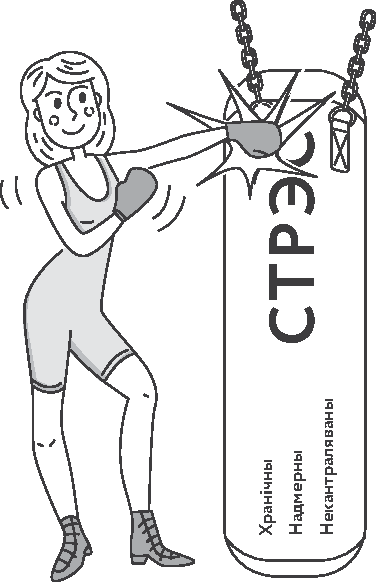
\includegraphics[scale=1.1]{willpower/ch7/1.pdf}
\end{figure}

\subsection*{Сацыяльны стрэс}

Людзі~--- істоты сацыяльныя, для нас быць у~калектыве~--- значыць выжыць. У старажытнасьці чалавек, адрынуты племем, асуджаны на выгнаньне, быў вырачаны. Таму мы і цяпер такія ўспрымальныя да сацыяльнага стрэсу. Сацыяльны боль часьцяком нашмат горшы за фізычны~--- бо фізычны мы перажываем адзін раз, а~сацыяльны не слабее: публічнае прыніжэньне мы згадваем шматкроць.

\emph{Да ліку стрэсараў, важных для выжываньня, мозг адносіць аспэкты SCARF: status, certainty, autonomy, relatedness, fairness, г. зн. статус, упэўненасьць, самастойнасьць, агульнасьць і справядлівасьць. Нас чапляе несправядлівасьць у~стаўленьні нас: калі хтосьці замахваецца на наш аўтарытэт, мы можам рэагаваць вельмі хваравіта.}

Мы міжвольна і эмпатычна можам капіяваць стрэс у~навакольных праз работу люстраных нэўронаў. Навукоўцы кажуць, што стрэс можа быць «заразны», і картызол узрастае, нават калі вы назіраеце за перажываньнямі іншых людзей. Цікава, што дэдлайн зьніжае эмпатычнасьць і ўспрыманьне чужога стрэсу.

\subsection*{Псыхалягічны стрэс}

У жывёлаў стрэс мае фізычны характар, узьнікае, калі выжываньню пагражае прамая небясьпека, і адносна рэдкі ў~іх жыцьці. А вось чалавек можа запускаць такую ж рэакцыю на ўяўныя пагрозы, якія малюе розум. Другая праблема ў~працягласьці рэакцыі: драпежнік гоніцца за жывёлай ня больш за хвіліну, тут ужо ці цябе зьелі, ці ты ўцёк, у~любым выпадку доўга турбавацца няма пра што. У чалавека ж псыхалягічны стрэсар можа дзейнічаць днямі і месяцамі, не паніжаючы інтэнсіўнасьці. У жыцьці цывілізаваных людзей дамінуюць менавіта псыхалягічныя стрэсары, таму пагражае нам не сама стрэсавая сытуацыя, а~рэакцыя на яе ці нават яе чаканьне, напрыклад страх звальненьня. 

\textbf{Мы можам сотню разоў пракручваць і перажываць складаную сытуацыю, прымушаючы сваё цела зноў і зноў рэагаваць на яе, што вельмі шкодна для здароўя.}

Псыхалягічны ціск складаецца з~сотняў дробязяў: праблемы ў~стасунках і на працы, асьцярогі рознага кшталту, нездаволеныя жаданьні і інш. Чым горш мы спраўляецца, тым мацнейшы на нас ціск, і наша адаптыўная сыстэма перастае вытрымліваць нагрузку. Кожны стрэсар узмацняе наш трывожны стан, а~наш трывожны стан становіцца больш адчувальным да кожнага новага стрэсара.

\emph{Ёсьць усходняя прыпавесьць пра люстраны пакой у~палацы шаха, які даваў дзясяткі адлюстраваньняў. Аднойчы туды забег сабака, які ўбачыў вакол мноства сабак, шчэрыў зубы, брахаў і кідаўся на люстэркі, адлюстраваньні шчэрыліся ў~адказ, а~рэха толькі ўзмацняла ягоны брэх. Раніцай служкі знайшлі ў~пакоі мёртвага сабаку, хоць у~люстраным пакоі не было нікога, хто мог бы яму нашкодзіць. Так і мы часта мацней пакутуем ад сваёй рэакцыі на думкі, жаданьні, пачуцьці, а~не ад прамога дзеяньня навакольных стрэсараў.}

\infobox{Вялікае значэньне маюць псіхалагічныя ўсталёўкі: ад таго, як вы ацаняеце стрэсар, залежыць ваша фізіялагічная рэакцыя на яго і ваша магчымасць да яго адаптавацца.}

Што ж ёсьць стрэсам? Адзін і той жа чыньнік для кагосьці можа быць стрэсарам, а~для іншага~--- не. Спартовец лёгка падымае вагу, здольную траўмаваць пачаткоўца, дасьведчаны перамоўца спакойна сьпіць пасьля канфлікту, які б ня даў заснуць усю ноч звычайнаму чалавеку. Тое, што для нас зьяўляецца ці не зьяўляецца стрэсарам, шмат у~чым залежыць выключна ад нашых рэсурсаў і навыкаў. Калі вы ўмацоўваецеся, ранейшая нагрузка выклікае ў~вас ужо не стрэс, а~толькі подзіў. Вялікае значэньне маюць псыхалягічныя ўстаноўкі: ад таго, як вы ацэньваеце стрэсар, залежыць вашая фізыялягічная рэакцыя на яго і вашая магчымасьць да яго адаптавацца.

Узьдзеяньне стрэсу на арганізм залежыць і ад іншых рэсурсаў здароўя. Напрыклад, пры стрэсе павышаецца артэрыяльны ціск, расьце ўзровень тлушчаў і глюкозы ў~крыві~--- і гэта зьяўляецца рызыкай сардэчна-сасудзістых захворваньняў і дыябэту. Але калі вы займаецеся спортам, то вашыя цягліцы лёгка спаляць лішак тлушчаў і глюкозы, а~яшчэ пры руху выдзяляецца аксід азоту, які зьмяншае артэрыяльны ціск. Так актыўнасьць абараняе вашае цела ад стрэсу. А вось калі ў~стане стрэсу вы лежыце на канапе перад тэлевізарам і заядаеце яго піцай, гэта яшчэ мацней павялічвае ўсе рызыкі.

Нягледзячы на тое, што ў~гэтым разьдзеле ўвесь час выкарыстоўваецца слова «стрэс», я б рэкамэндаваў менш ужываць яго ў~адносінах да свайго жыцьця. Кажучы «стрэс», мы як быццам ставім сабе дыягназ невылечнай хваробы, зь якой трэба зьмірыцца й жыць. Лепш скажыце сабе, маўляў, у~мяне ёсьць задача ці праблема, што выклікае ў~мяне пэўныя рэакцыі. І калі гэта задача, дык яе можна прааналізаваць і вырашыць, а~ня «вытрываць».

\emph{\textbf{Зрабіць зь лімонаў ліманад.} Мне падабаецца мэтафара з~гештальт-тэрапіі: стрэс~--- гэта ежа. Чым гастрэйшыя вашыя зубы і мацнейшыя сківіцы, тым мацнейшы стрэс вы можаце ня проста перажаваць, але й засвоіць ягоныя карысныя ўласьцівасьці. Любыя падзеі як ежа~--- ці зможаце вы іх перастрававаць? Слушна заўважалі стоікі: «Нашыя дзеяньні могуць сутыкацца зь перашкодамі, але для нашых намераў ці плянаў перашкодаў не існуе. Бо мы здольныя падладжвацца і прыстасоўвацца. Сьвядомасьць прыстасоўваецца і абяртае на сваю карысьць перашкоду, якая стала на шляху нашых дзеяньняў. Перашкода на шляху дзеяньня спрыяе дзеяньню. Тое, што стаіць на шляху, становіцца шляхам». Марк Аўрэлій, 170 год н.э.}

\subsection*{Пытаньні і заданьні}

1. Ці гатовыя вы адхапіць «свой кавалак» ад жыцьця, адаптаваўшыся да новых умоваў? Ці вы лічыце, што мусіць зьмяніцца сам сьвет?

2. Успомніце сытуацыі, якія былі стрэсавымі для вас у~мінулым, а~цяпер вы лёгка даяце ім рады. Што дапамагло вам зьнізіць іх стрэсагеннасьць?

3. Якая ваша самая тыповая рэакцыя на стрэс? Ударыць, уцячы, замерці, дрыжаць? Ці дапамагае яна вам? Ці ўдавалася вам зьмяніць сваю тыповую рэакцыю?


\section{Уплыў стрэсу на здароўе}

Прымаўка сьцьвярджае, што «ўсе хваробы ад нэрваў, і толькі некаторыя~--- ад задавальненьня». Які стрэс найбольш небясьпечны? Той, што выклікае зьнясіленьне, якім мы не можам кіраваць. Замест адаптацыі такі стрэс выклікае страту рэсурсаў, выгараньне, зьнясіленьне, аж да дэпрэсіі. Гэта суправаджаецца адчуваньнем катастрофы, стратай сэнсу і задавальненьня ў~жыцьці. Небясьпечная не аднаразовая стрэсавая рэакцыя, а~менавіта сыстэматычнае ўзьдзеяньне на працягу доўгага часу: «шкодны» стрэс мае выразны назапашвальны эфэкт. У сучасным жыцьці мы сутыкаемся зь лішкам стрэсу эмацыйнага, некантраляванага, хранічнага, і пры гэтым нам можа бракаваць гострага стрэсу.

\emph{Гостры стрэс, такі як фізычная актыўнасьць, хоць і павялічвае ціск, але трэніруе сэрца~--- у~выніку спорт зьніжае ціск і пульс у~стане спакою, што зьяўляецца спрыяльным і карысным.}

Для нашых далёкіх продкаў стрэс быў зьвязаны з~прамой пагрозай для жыцьця, для выжываньня даводзілася разьвіваць фізычную актыўнасьць і эканоміць энэргію. Таму пры стрэсе запускаюцца рэакцыі, якія павышаюць гатоўнасьць да фізычнай актыўнасьці (рэакцыя «бі~--- бяжы»): павялічваецца ціск, пульс, пачашчаецца дыханьне, павялічваецца цяглічны тонус і канцэнтрацыя ў~крыві глюкозы і тлушчаў. Калі такая рэакцыя запускаецца занадта часта, а~пры гэтым мы шмат сядзім, то яна шкодзіць нам: павышэньне цукру павялічвае пашкоджаньне сасудаў і павышае рызыку дыябэту, павышэньне тлушчаў правакуе зьяўленьне атэрасклерозу, павышэньне ціску павялічвае рызыку сардэчна-сасудзістых захворваньняў і да т.~п.

\subsection*{Хранічны стрэс і энэргія}

Пры стрэсе арганізм пачынае запасіць энэргію, бо хранічны стрэс часта быў зьвязаны з~голадам. Таму ў~нас узмацняецца апэтыт, назапашваецца тлушч, адключаюцца «няважныя» палавая сыстэма, шчытавіца, імунітэт, касьцяная сыстэма~--- усё дзеля эканоміі энэргіі. \textbf{Калі гаворка ідзе пра выжываньне, то нам, вядома, не да размнажэньня.}

Разьвіваецца гіпадынамія~--- і гэта не «сьвядомае» нежаданьне рухацца, першаснае тут менавіта прыгнечаньне жаданьня руху мозгам. Пры гэтым чым менш мы рухаемся і больш ямо, тым яшчэ вышэйшая рызыка дэпрэсіі і яшчэ ніжэйшыя рэсурсы~--- так фармуецца замкнёнае кола.

\subsection*{Стрэс і запаленьне}

Стрэс павялічвае ўзровень запаленьня. У выпадку нападу або ўцёкаў звычайна здараюцца раненьні, у~раны могуць трапіць бактэрыі, таму важна загадзя павысіць актыўнасьць запаленчай рэакцыі~--- так эвалюцыйна арганізм прывык рэагаваць на стрэс. Таму пры стрэсе арганізм «па звычцы» назапашвае вадкасьць і натрый, павялічвае актыўнасьць сыстэмы згортваньня і ўзровень запаленчых малекулаў. У бойцы гэта дапамагло б справіцца са стратай крыві і хутчэй загаіць раны. У звычайным мірным жыцьці гэта толькі павялічвае нашы рызыкі: напрыклад, чым вышэйшы ўздым запаленчага маркера С-рэактыўнага бялку, тым вышэйшая рызыка разьвіцьця постстрэсавай дэпрэсіі.

\subsection*{Рэгуляцыя стрэсу}

Стрэсавая сыстэма мае шмат \textbf{узроўняў рэгуляцыі}. На гарманальным узроўні працуюць гармоны картызол і адрэналін, ім дапамагае вэгетатыўная нэрвовая сыстэма. Яна складаецца са стрэсавай сімпатыйнай і антыстрэсавай парасімпатыйнай сыстэмаў, гэта як газ і тормаз у~аўтамабілі. 

\infobox{Гіпэрактыўнасьць сімпатыйнай нэрвовай сыстэмы пагаршае шкоду стрэсу, а, стымулюючы парасімпатычную сыстэму, мы можам заўважна прыслабіць дзеяньне стрэсу на наш арганізм.}

\emph{Некантраляваны гостры стрэс празьмернай сілы павялічвае рызыку сьмерці. Напрыклад, крах біржы, як і землятрус, павялічвае ў~найбліжэйшыя дні сьмяротнасьць ад сардэчна-сасудзістых захворваньняў. Нават пройгрыш любімай каманды можа павысіць сьмяротнасьць, а~вось выйгрыш можа зьнізіць рызыку сьмяротнасьці бліжэйшымі днямі~--- такая адказнасьць перад заўзятарамі. Пастаноўка дыягназу «рак» павялічвае рызыку сардэчна-сасудзістай сьмерці ў~першы тыдзень амаль у~шэсьць разоў, у~першы месяц~--- у~тры разы, а~да канца года рызыка становіцца сярэдняй.}

Стрэс нэгатыўна ўплывае на працу мозгу, зьніжае нэўраплястычнасьць, сінаптагенэз, нэўрагенэз, што вядзе да пагаршэньня памяці і павелічэньня рызыкі дэмэнцыі. Хранічныя стрэсы фізычна зьмяншаюць памер мозгу, пакутуюць найважнейшыя структуры мозгу: гіпакамп (памяншаецца на 7--15\,\%) і кара лобных доляў. Вобласьці прэфрантальнай кары адказваюць за самакантроль, а~чым горшы самакантроль~--- тым горш вы даяце рады са стрэсам. І зноў фармуецца заганнае кола.

\subsection*{Стрэс і сэрца}

\textbf{Стрэс адмоўна ўзьдзейнічае на сэрца}: узмацняе працу сімпатыйнай нэрвовай сыстэмы, пагаршае кровазабесьпячэньне, правакуе разьвіцьцё арытмій, стымулюе згусаньне крыві і г.~д. Чым больш напругі на працы, тым вышэйшая рызыка атэрасклерозу каранарных сасудаў і падвышанага ціску. У Японіі нават існуе тэрмін «каросі»~--- сьмерць (інсульт або інфаркт) на працоўным месцы ад перапрацоўкі. Высокі ўзровень перажытага стрэсу летась у~чатыры разы павялічвае рызыку інсульту. А ўсяго некалькі месяцаў перапрацоўкі па 10 гадзінаў за дзень на траціну павялічваюць імавернасьць інсульту.

\emph{Праграмы зьніжэньня стрэсу пасьля інфаркту прыводзяць да зьніжэньня сьмяротнасьці ў~бліжэйшы год назіраньня, а~праграма рэляксацыі на працягу 6--9 месяцаў зьніжае ня толькі стрэс, але й ягоныя наступствы~--- зварочвае атэрасклероз, прыводзіць да памяншэньня таўшчыні інтым-мэдыя сонных артэрыяў, зьніжае ЧСС, павышае варыябэльнасьць сардэчнага рытму, паляпшае пераноснасьць фізычнае нагрузкі, зьніжае частасьць прыступаў стэнакардыі, эпізодаў арытміі, а~таксама колькасьці сьмерцяў ад ССЗ.}

Стрэс зьніжае адчувальнасьць да інсуліну і павялічвае рызыку дыябэту. Стрэсавае пераяданьне пагаршае гэты працэс. Пры стрэсе лішак картызолу ўзмацняе страту цяглічнай масы і павялічвае набор тлушчу ў~вобласьці жывата, правакуючы вісцэральнае атлусьценьне, а~таксама ў~верхняй частцы цела, уключаючы твар і шыю. Хранічны стрэс пагаршае структуру цела, прыводзячы да ўтварэньня ў~розных частках цела «пастак тлушчу», устойлівых да пахуданьня. Стрэс вядзе да парушэньня працы імуннай і стрававальнай сыстэмаў, прама ці ўскосна шкодзіць усяму арганізму. Стрэс кароціць тэламэры, а~чым карацейшыя тэламэры, тым вышэйшая хуткасьць старэньня.

\subsection*{Стрэс і нездаровыя паводзіны}

Як трапна заўважыў Ірвін Ялам: «Чалавек не выбірае сваю хваробу, але ён выбірае стрэс~--- і менавіта стрэс выбірае хваробу». Бадай, найболей небясьпечным зьяўляецца тое, што стрэс робіць чалавека больш імпульсіўным і звужае гарызонт плянаваньня. Чалавек пачынае для расслабленьня заядаць стрэс, які і сам па сабе ўзмацняе цягу да высокакалярыйнай ежы і дазваляе зьесьці неймаверную колькасьць ежы без адчуваньня насычэньня. Стрэс узмацняе цягу да нікатыну, алькаголю, іншым наркотыкам, азартным гульням, рызыкоўным паводзінам, залежным адносінам. Фармуецца нездаровая мадэль паводзінаў: пры стрэсе мы «ўзнагароджваем» сябе смачным, і гэта замацоўвае паводзіны «лузэра». Пакуль мы знаходзімся ў~стане стрэсу і не рашылі задачу, варта пазьбягаць узнагародаў любога кшталту. Ёсьць рызыка пачаць змагацца стымулятарамі з~такімі стрэсавымі сымптомамі, як стома або ангеданія, актыўна нарошчваючы іх дозы. У рэшце рэшт гэта прывядзе толькі да большага спусташэньня. 

\begin{figure}[htb!]
  \centering
  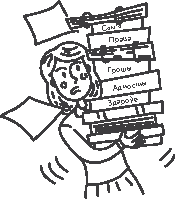
\includegraphics[scale=1.5]{willpower/ch7/2.pdf}
\end{figure}

\infobox{У стане стрэсу вялікая рызыка зрыву і вяртаньня да ранейшых нездаровых мадэляў паводзінаў, таму, калі вы былі залежныя ад ежы, алькаголю ці курэньня, будзьце асабліва пільныя.}

Скарачэньне HALT(S) часта выкарыстоўваецца ў~прафіляктыцы і лячэньні залежнасьцяў як трыгеры зрыву. Hungry (галодны), angry (злы), lonely (самотны), tired (стомлены), S ёсьць некалькі Sad Sick Stressed Serious (сумны, стрэсаваны, сур'ёзны)~--- гэта трыгеры, якія запускаюць непажаданыя паводзіны і прыводзяць да таго, што мы прымаем няправільныя рашэньні і можам сарвацца. Калі вы знаходзіцеся ў~адным з~гэтых станаў, то лепш устрымацца ад высноваў, словаў і дзеяньняў. Бо гэтыя станы вельмі моцна ўплываюць на працэс мысьленьня, скажаючы яго, і гэтае скажэньне нам цяжка заўважыць. Спачатку трэ выправіць стан (паесьці, супакоіцца, пагутарыць, адпачыць), а~затым~--- прымаць рашэньні.

\subsection*{Мысьленьне і стрэс}

Актыўнасьць прэфрантальнай сыстэмы залежыць ад шматлікіх чыньнікаў~--- стрэсы, недасып, разумовая і фізычная перагрузка, выгараньне саслабляюць яе. Аслабленьне агульнага здароўя, гарманальны дысбалянс, дэфіцыт сонечнага сьвятла або зьбедненае асяродзьдзе~--- усё гэта зьніжае яе сілу. Акрамя агульнага зьніжэньня разумовай прадукцыйнасьці, адбываецца і сёе-тое горш: аслабляецца тармазны кантроль над падкоркавымі цэнтрамі, уключаючы мігдаліну, прылеглае ядро і да т.~п. Растармажэньне вядзе да фэномэну «блуканьня розуму», якое на фоне стрэсу і стомы афарбоўваецца нэгатывам, бо ў~стане стрэсу значнасьць нэгатыўных чыньнікаў вышэйшая і яны аўтаматычна прыцягваюць увагу.

\emph{Як гэта адбываецца? Спачатку ваша ўвага адзьдзяляецца ад вонкавых чыньнікаў і перанакіроўваецца на ўнутраную плынь інфармацыі, затым паніжаецца кантроль над сэнсавым зьместам сьвядомасьці, узмацняецца выманьне інфармацыі з~памяці і ўсе мэты мысьленьня становяцца асабіста і эмацыйна афарбаванымі. Калі нэгатыўная думка ці эмоцыя прыходзіць, прэфранталка павінна зь ёй нешта зрабіць, неяк адрэагаваць.}

Прэфрантальная кара мозгу~--- гэта інструмэнт, як Google. «Окей, Гугл, чаму мне кепска?» І вы атрымліваеце сотні й тысячы магчымых прычынаў, разгляд якіх («зварот да памяці») прымушае зноўку перажываць нэгатыўны вопыт і яшчэ мацней закручвае сьпіраль нэгатыву.

У стрэсе ў~нас скача фокус увагі, адбываецца аўтаматычнае абмежаваньне ўспрыманьня інфармацыі, не зьвязанай з~выжываньнем, нам цяжка адрозьніваць дэталі, бо ўзмацняецца палярызацыя мысьленьня (чорна-белае ўспрыманьне), пагаршаюцца пэўныя кагнітыўныя навыкі, памяншаецца здольнасьць улічваць наступствы сваіх дзеяньняў, узмацняецца стэрэатыпнасьць, могуць паўстаць фэномэн блякады мінулага досьведу і тунэльнае ўспрыманьне і яшчэ шмат іншых багаў. Самае непрыемнае ў~гэтых багах~--- мы ня можам заўважыць іх знутры, то бок знаходзячыся ў~стане стрэсу.

\subsection*{Ня ўсім сваім думкам вер}

Адным з~найважнейшых для мяне адкрыцьцяў ва ўсьвядомленасьці стаў навык адрозьніваць «слабыя» думкі, выкліканыя стрэсам і рэакцыяй на эмоцыі, ад маіх «моцных», сапраўдных думак, якія адлюстроўваюць рэальнасьць і мае асабістыя ўстаноўкі. Усьвядомленасьць дапамагае зразумець, што «слабыя» думкі~--- гэта толькі «ўнутраная прапаганда», рэакцыя на нерэалістычную ўнутраную карціну сьвету, фэйк. Калі мы сур'ёзна рэагуем на «слабыя» думкі, то ўспрымаем сваю слабасьць пасьля ГРЗ за слабахарактарнасьць, варожае ўспрыманьне іншага чалавека праз недасып як яго рэальную ацэнку, страх перад пачаткам праекта празь нізкі тэстастэрон за сваё прыроджанае няўменьне канкураваць. 

Якая з~гэтага выснова? З эмоцыямі ня варта «лягічна разьбірацца», калі яны зьяўляюцца толькі прадуктам вашага стрэсу, недасыпу, хваробы, г.~зн. адлюстраваньнем «слабога» стану зь нізкім кагнітыўным кантролем і неадэкватным успрыманьнем рэальнасьці. Важна ў~кожны момант разумець, што нашае мысьленьне залежыць ад стану розуму і цела. Чым вы слабейшыя фізычна, чым горшы кантроль увагі, тым горшае і кіраваньне падкоркай. Усьвядомленасьць, вядзеньне дзёньніка дазваляе заўважыць, як моцна мяняецца хада вашых думак у~залежнасьці ад узроўню энэргіі.

\emph{Спытайце сябе: мае думкі проста цяпер~--- гэта рэальнасьць ці прадукт сьвядомасьці або стрэсу? Ёсьць клясычная мадэль успрыманьня АВС, дзе А~--- рэальная сытуацыя (як быццам запіс відэа), В~--- яе інтэрпрэтацыя сытуацыі (ацэначнае меркаваньне), С~--- нашыя рэакцыі ды імпульсы. Так мы можам асобна разгледзець усе кампанэнты нашага ўспрыманьня і ўбачыць неадпаведнасьці.}

\begin{figure}[htb!]
  \centering
  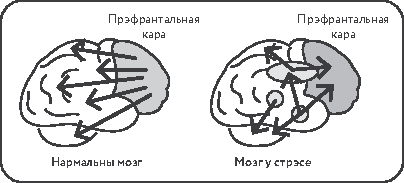
\includegraphics[scale=1.15]{willpower/ch7/3.pdf}
\end{figure}

\textbf{Верце думкам у~моцныя моманты.} Важна даваць ацэнкі, прымаць рашэньні, плянаваць, весьці перамовы толькі ў~тыя моманты часу, калі ваша прэфранталка ў~найлепшай форме~--- як правіла, гэта ранішні час. На працягу тыдня імкніцеся заставацца ў~форме, сочачы за рэжымам і ўзроўнем актыўнасьці, каб як мага больш гадзінаў былі «моцнымі». Усё, што дапамагае палепшыць здароўе, аптымізаваць біямаркеры, умацаваць стрэсаўстойлівасьць~--- усё гэта павышае колькасьць «моцных» гадзінаў. Важны навык адрозьніваць «слабыя» думкі, выкліканыя стрэсам і рэакцыяй на эмоцыі, ад «моцных», сапраўдных думак, якія адлюстроўваюць рэальнасьць і асабістыя ўстаноўкі.

\subsection*{Вымярайце стрэс}

Рыпеньне можа напалохаць нас толькі ў~цемры, а~ня ў~сьветлым пакоі. Так і стрэс палохае нас, калі ён незразумелы. Пачніце вывучаць стрэс, і ўжо гэта аслабіць ягонае ўзьдзеяньне. Можна спалучаць розныя спосабы, бо ніводны зь іх не дасканалы. Возьмем аналіз стрэсу: можна здаць у~лябараторыі шэраг стрэсавых паказьнікаў, напрыклад профіль картызолу або альфа-амілазу сьліны, можна з~дапамогай датчыка маніторыць варыябэльнасьць пульсу, праходзіць апытанікі і ацэньваць як стрэсар, так і сваю рэакцыю на яго.

Важна ўмець назіраць, і найлепшы спосаб для гэтага~--- весьці \textbf{дзёньнік стрэсу}. Адзначайце, як вы рэагуеце на стрэсавы дзень: затор, складаная размова, таксічны калега, бессань, сьпешка,~--- і ацэньвайце, што вам дапамагае, а~што яшчэ больш узмацняе стрэс. Зь якімі стрэсарамі вы сустракаецеся часта і яны сталі для вас звыклымі, а~якія стрэсары рэдкія ў~вашым жыцьці? 

\textbf{Адсочвайце рэакцыі на кожны ўзьніклы стрэсар:} 
\begin{itemize}
  \item фізыялягічныя рэакцыі: потадзьдзяленьне, пачашчаны пульс, цяглічная напруга;
  \item псыхалягічныя рэакцыі: страх, турбота, зьбянтэжанасьць, скрайняе хваляваньне. 
\end{itemize}

\textbf{Ацаніце свае спосабы адаптацыі да стрэсара}, прыёмы рэляксацыі, скарыстаныя ў~гэты дзень, і іх эфэктыўнасьць. Адзначайце адчуваньні на працягу дня: фізычныя, напрыклад, галаўны боль, боль у~страўніку ці ў~сьпіне, і псыхалягічныя, напрыклад, прыступ неспакою, пачуцьцё няўпэўненасьці, адчуваньне цэйтноту.

\textbf{Ацаніце сваю стрэсавую рэакцыю:}
\begin{itemize}
  \item парог рэакцыі: які стымул якой сілы выклікае ў~вас стрэс;
  \item велічыня рэакцыі: як вы рэагуеце;
  \item хуткасьць згасаньня і аднаўленьня пасьля стрэсу: чым хутчэй вы вяртаецеся ў~норму, тым вышэйшыя вашыя рэсурсы.
\end{itemize}

У інтэрнэце можна знайсьці вялікую колькасьць карысных апытанак, якія дапамогуць ацаніць вашую рэакцыю на стрэс і індывідуальныя асаблівасьці. Вы можаце зразумець, да якіх копінг-стратэгіяў зьвяртаецеся часьцей за ўсё, які ў~вас тып паводзінаў: тып А~--- сімпатыйны, або тып Б~--- парасімпатыйны.

\textbf{Варыябэльнасьць сардэчнага рытму} можна вымяраць з~дапамогаю бранзалета, датчыка, тэлефона, вымяраюцца шмат паказьнікаў, напрыклад SDNN, RMSSD, pNN50. Чым вышэй варыябэльнасьць пульсу, тым лепш. Разьлічваюцца і вытворныя: хвалі з~высокай частатой HF паказваюць актыўнасьць парасімпатыйнай сыстэмы, а~зь нізкай LF~--- сімпатыйнай. Калі мала HF, то брак расслабленьне, калі мала LF~--- то нізкі тонус. Суадносіны LF / HF характарызуе вэгетатыўны балянс.

\subsection*{Пытаньні і заданьні}

1. Як хутка вы вяртаецеся ў~норму пасьля перажытага стрэсу? (Чым хутчэй, тым лепш.)

2. Як мяняецца вашае ўспрыманьне сьвету, сябе і іншых людзей у~момант стрэсу?

3. Як стрэс уплывае на вашыя паводзіны і якія шкодныя звычкі ён у~вас правакуе? Пачніце весьці дзёньнік стрэсу, каб заўважыць гэта.


\section{Стрэс і энэргія}

Гостры стрэс можа зарадзіць нас энэргіяй, і стрэсавую падзею мы можам утаймаваць як неаб'езджанага жарабца. Хранічны ж стрэс~--- ён як паразіт, павольна высмоктвае сілы і энэргію з~дня ў~дзень. Як мы ўжо гаварылі, стрэсаўстойлівасьць непасрэдна зьвязаная з~нашым узроўнем энэргіі і колькасьцю рэсурсаў. Чым менш у~нас энэргіі, тым горш мы супрацьстаім стрэсу і тым менш у~нас застаецца энэргіі~--- узьнікае замкнёнае кола. Доўгае ўзьдзеяньне стрэсараў, кепскае аднаўленьне і нізкія рэсурсы прыводзяць да перагрузкі і зьнясіленьня, а~гэта зьмяншае ўзровень даступнай нам энэргіі, якую мы можам накіраваць на вырашэньне сваіх праблемаў. 

\infobox{Многія людзі, якія хочуць зьмяніць сваё жыцьцё, ня могуць гэтага зрабіць проста таму, што не валодаюць дастатковым узроўнем энэргіі.}

\textbf{Канцэпцыя «аластатычнай нагрузкі»} стрэсу кажа аб працяглым залішнім узьдзеяньні стрэсавых чыньнікаў, якія маюць назапашвальны нэгатыўны эфэкт. Калі нагрузка занадта вялікая, у~арганізьме ўзьнікае канкурэнцыя паміж рознымі працэсамі. Можа бракаваць рэсурсаў на аднаўленьне або на імунітэт, бо прыярытэтам пры стрэсе зьяўляецца кароткатэрміновае выжываньне, а~доўгатэрміновыя наступствы аказваюцца ня так важныя. У рэшце рэшт назапашаная стрэсавая нагрузка вядзе да паломкі ў~самым уразьлівым месцы арганізма. Чым болей у~вас стрэсу, тым меней сілаў, а~чым меней сілаў, тым меншая гатоўнасьць супрацьстаяць стрэсу.

\textbf{Псыхалягічныя рэсурсы}~--- гэта як праграмы для кампутара. Чым лепшыя праграмы, тым больш эфэктыўна мы адаптуемся і вырашаем складаныя жыцьцёвыя сытуацыі. Да ліку такіх рэсурсаў можна аднесьці самакаштоўнасьць, самакантроль, самапавагу, прафэсійныя кампэтэнцыі, сацыяльнае асяродзьдзе, сям'ю, даход~--- усё, што прама або ўскосна павялічвае выжываньне ды імавернасьць дасягненьня мэтаў. Павялічваючы, пісьменна аднаўляючы і пераразьмяркоўваючы свае рэсурсы, мы пачынаем лягчэй прыстасоўвацца. 

\textbf{Таму разьвіцьцё стрэсаўстойлівасьці і ўключае ў~сябе самыя розныя навыкі~--- гэта ня проста пра «ўмець адпачываць».} Галоўным рэсурсам звычайна выступае самакантроль і самаарганізацыя, якія кантралююць і арганізуюць разьмеркаваньне іншых рэсурсаў і мацней за ўсё падаюць пры стрэсе.

\subsection*{Варонка зьнясіленьня} Калі мы пасьпяхова адольваем адну задачу, то ўпэўненыя, што можам адразу пацягнуць такую ж ці яшчэ больш складаную, забываючы пра неабходнасьць аднаўленьня сілаў. Шкодная прынятая ў~культуры «гераізацыя працы» і небясьпечныя для здароўя віды работ, дзе да супрацоўнікаў выстаўляюцца высокія патрабаваньні, але забясьпечваецца нізкая падтрымка. Часта прафэсійная дзейнасьць страчвае часавыя рамкі, адцягвае і раніцай, і ўвечары. Каб лепей спраўляцца з~працай, мы менш адпачываем і пачынаем скарачаць «непатрэбную» актыўнасьць: сустрэчы, хобі, забаўкі. 

\infobox{Парадокс: чым больш мы прыбіраем сілкавальныя для нас заняткі, тым меней у~нас застаецца сілаў.}

Зьнясіленьне неўпрыкметаў выклікае страту задавальненьня ад жыцьця, разьвіваецца ангеданія. Нам усё меней хочацца нешта рабіць, узьнікае раздражняльнасьць, звужэньне кола кантактаў, пракрастынацыя, мяняецца сон, становіцца менш спантаннасьці й лёгкасьці ў~паўсядзённым жыцьці, зьнікае жаданьне рабіць нават рутынныя справы. Узьнікае своеасаблівая сьпячка, якая суправаджаецца пачуцьцём хранічнае стомы~--- калі працяглы адпачынак перастае прыносіць палёгку, у~адрозьненьне ад назапашанай стомы, калі адпачынак яшчэ дапамагае. Хранічны стрэс і нездаровы лад жыцьця могуць прывесьці і да мэтабалічных парушэньняў, разьвіцьця своеасаблівага «рэжыму дэфіцыту», пры якім усе працэсы скіраваныя на эканомію энэргіі і выжываньне. Калі людзі не выкарыстоўваюць свае навыкі, то пачынаюць іх страчваць: зьмяншаюцца цяглічная маса, кагнітыўныя здольнасьці, стрэсаўстойлівасьць і шматлікае іншае.

\subsection*{Стратэгія назапашваньня энэргіі} Пры хранічным стрэсе ўзьнікае звычка жыць адным днём. Людзі заклапочаныя здыманьнем стрэсу, бо рэальнасьць такая невыносная. Стрэс можна здымаць ілюзіямі або дафамінавай «халявай»: рызыкоўнымі паводзінамі, гіпэркалярыйнай ежай, алькаголем, азартнымі гульнямі, наркотыкамі і да т.~п. Такі нездаровы лад жыцьця і стымуляцыя на час могуць падняць настрой і энэргію, але забіраюць сілы і энэргію ў~заўтрашняга дня, узмацняючы стрэс. Пачаць назапашваньне энэргіі варта з~увядзеньня антыстрэсавага рэжыму. Праца са стрэсам індывідуальная: залежыць ад генэтыкі, асабістых асаблівасьцяў, тыпу стрэсара, акалічнасьцяў і даступных вам рэсурсаў. Часта дапамагае нават зьмена ацэнкі сытуацыі. Зьмяніўшы бачаньне, можна зьмяніць і фізыялягічную рэакцыю на стрэсар, вызначыўшы яго як «не пагрозьлівы».

Чым мацней вы будзеце прымушаць сябе штосьці рабіць, тым вышэй будзе стрэс і, верагодна, гэта ня пойдзе вам на карысьць. Велізарныя пляны могуць сарваць усю распачатую працу над сабой, таму пачынаць трэба зь невялікіх крокаў.

\textbf{Моцны стрэс дае інфармацыю ў~катэгарычнай форме: «Такім займацца нельга! Гэтага трэба пазьбягаць любым коштам!»} Таму зону камфорту варта пашыраць паступова, дамагаючыся невялікіх зьменаў. Як толькі вы страчваеце цікавасьць ці адчуваеце агіду, варта спыніць заняткі: спорт, дыета ці вывучэньне новага навыку варта рабіць «па любові». Важна дадаць у~кожны працэс задавальненьне, атрымліваючы кайф ад пераадоленьня сябе, ад прыгожага спартовага адзеньня або сэрвіроўкі стала. Рэгулярнасьць нават малых перамог і захаваньне рэжыму важныя для павелічэньня ўпэўненасьці ў~сабе, што дасьць вам сілы для далейшага прагрэсу. Разглядайце свае заняткі як інвэстыцыю ў~будучыню, бо карысьць~--- гэта і ёсьць задавальненьне ў~будучыні.

\subsection*{Рэсурсы энэргічнасьці}

Усе рэсурсы энэргічнасьці мы можам умоўна падзяліць на цэнтральныя і пэрыфэрычныя. Да цэнтральных можна аднесьці прэфрантальную кару, дафамінавую сыстэму і цэнтры, якія адказваюць за стрэс. Розныя дафамінавыя праблемы, ад залежнасьцяў да фрустрацыяў, забіраюць вельмі шмат энэргіі. Таму такія важныя ўсьвядомленасьць і разуменьне таго, што менавіта ў~вашым жыцьці забірае энэргію і ўвагу, дзе вашыя «чорныя дзіркі».

\emph{Паспрабуйце ўпарадкаваць увагу. Прыбярыце паглынальнікі вашай увагі ў~жыцьці, факусуйцеся на сваіх плянах, думайце пра будучыню, практыкуйце ўдзячнасьць таму, што ёсьць цяпер. Разьбярыцеся з~інфармацыяй, якую вы «ўжываеце», і памятайце, што яна таксама сёе-тое есьць~--- вашую ўвагу! Што яшчэ крадзе энэргію? Часьцяком розныя крыўды, пачуцьцё віны, трывога, румінацыі могуць адымаць большую частку вашай энэргіі зусім непрадуктыўна.}

Даданьне спантаннасьці, навізны, гульні, крэатыўнасьці, разнастайнасьці ў~паўсядзённае жыцьцё дапаможа павысіць і ўзровень энэргіі. Варта паступова прыбіраць дафамінавую «халяву» (цукар, вугляводы, алькаголь, смартфон, балбатню) і дадаваць больш добрага дафаміну (хобі, масаж, камунікацыя, сонца, рух, перамогі і да т.~п.).

\textbf{Для адэкватнай працы мозгу неабходнае падсілкоўваньне задавальненьнем.} Наш настрой, матывацыя, энэргія залежаць ад нэўрамэдыятара дафаміну. Навык шчасьця~--- гэта атрыманьне задавальненьня зь ненаркатычных крыніцаў. Чым менш чалавек атрымлівае задавальненьня ад свайго паўсядзённага жыцьця, тым больш актыўна ён зьвяртаецца да вонкавай стымуляцыі. Калі дафаміну бракуе, то ўзьнікае «сындром дэфіцыту задаволенасьці»~--- калі вам цяжка атрымліваць задавальненьне ад паўсядзённых справаў, учынкаў, стасункаў. Усё перастае цешыць, акрамя магутных гіпэрстымулаў, часьцяком небясьпечных ці перакручаных, а~калі нешта кранае, хвалюе, то радасьць хутка зьнікае.

\emph{Праблема дэфіцыту задаволенасьці зьвязаная з~самымі разнастайнымі відамі залежнасьцяў: алькаголь, курэньне, інтэрнэт, залежныя стасункі, пераяданьне, агрэсія, рызыкоўныя паводзіны, наркатычныя залежнасьці, порназалежнасьць і інш.}

Чым мацней, часьцей і даўжэй вы стымулюеце сваю дафамінавую сыстэму задавальненьняў, тым меншую колькасьць дафаміну яна пасьля выпрацоўвае. Пасьля моцнай стымуляцыі любога кшталту назіраецца дысфарыя і ангеданія: лішак задавальненьняў у~любым выглядзе зьмяншае адчувальнасьць дафамінавых рэцэптараў, вядзе да страты смаку ад жыцьця, зьмяншае жаданьне дасягаць нечага. \textbf{Таму важна прытрымлівацца ўмеранай аскезы і абмежаваньняў~--- парадаксальна, але яны зробяць асалоды больш яркімі і дапамогуць вярнуць матывацыю.}

«Не дазваляйце сабе аніякіх глупотаў, акрамя тых, якія прынясуць вам велізарнае задавальненьне»: сёньня ў~тэрапіі пазітывам людзей вучаць атрымліваць задавальненьне ад плянаваньня, дзеяньня і навучаньня. Скараціце колькасьць справаў, якія вы ня хочаце рабіць, якія вам зусім не даспадобы, і дадайце больш справаў, якія павялічваюць настрой і якія вы робіце з~задавальненьнем. Вы загадзя плянуеце сабе задавальненьні, каб атрымліваць радасьць ужо ад іх прадчуваньня~--- я называю гэта «дафамінавым маяком»,~--- затым сьвядома атрымліваеце асалоду ад працэсу, пасьля гэтага дзеліцеся ўражаньнямі зь іншымі і разьвіваеце ўдзячнасьць ад перажытага. Радасьць лечыць і зараджае!

\textbf{Пэрыфэрычныя рэсурсы энэргічнасьці}~--- гэта ўсё, што знаходзіцца за межамі чарапной каробкі, гаворка як пра ўзьдзеяньне на цела, так і пра біяхімічныя аспэкты работы арганізма. Для таго каб выявіць магчымыя прычыны зьніжэньня энэргічнасьці на ўзроўні гармонаў і мэтабалізму, трэба правесьці шэраг дасьледаваньняў.

\emph{Парушэньні працы шчытавіцы (аналіз ТТГ, вольнага Т3), зьніжэньне тэстастэрону, павышэньне запаленьня (С-рэактыўны бялок і ІЛ-6), нізкі ўзровень жалеза (фэрытын), інсулінарэзістэнтнасьць і высокі глікаваны гемаглабін, лептынарэзыстэнтнасьць, высокі гомацыстэін (і нізкія ўзроўні B\textsubscript{9} і B\textsubscript{12}) могуць прыводзіць да зьніжэньня энэргічнасьці.}

Базавая нармалізацыя ладу жыцьця таксама вельмі важная. Напрыклад, гіпадынамія зьніжае энэргічнасьць, а~гармон голаду грэлін, наадварот, павялічвае і ўзровень дафаміну, і энэргічнасьць. Ясная рэч, бяз добрага сну тут не абысьціся.

\subsection*{Пытаньні і заданьні}

1. Як часта вы намаганьнем прымушаеце сябе нешта рабіць?

2. Якія праблемы са здароўем абмяжоўваюць вашу стрэсаўстойлівасьць?

3. Складзіце сьпіс «уцечак» вашай энэргіі, дзе розныя крыўды, трывогі зьядаюць вашыя сілы.


\section{Антыстрэсавы рэжым}

\textbf{Антыстрэсавы рэжым}~--- гэта своеасаблівы стрэсавы тайм-мэнэджмэнт, у~якім важна пазьбягаць зьнясіленьня, правільна разьмяркоўваць рэсурсы, надаваць дастатковы час аднаўленьню. Правільны выразны рэжым дня з~рэжымам харчаваньня, руху і сну вельмі важны для назапашваньня сілаў. Варта перагледзець свае задачы, прыбраць тыя, што мардуюць вас, і павялічыць тыя, што сілкуюць.

\infobox{Завядзіце антыдзёньнік, у~які першымі ўносіце паўзы, адпачынак, рэлаксацыю і толькі пасьля гэтага~--- справы!}

Ніцшэ неяк заўважыў, што «той, хто ня можа ўкладвааць 2/3 дня асабіста для сябе, павінен быць названы рабом». Але сучасныя дасьледаваньні паказваюць, што для адчуваньня шчасьця працоўнаму чалавеку трэба дзьве з~паловай гадзіны часу для сябе. Бо, з~аднаго боку, яго лішак вядзе да таго, што людзі адчуваюць бязмэтнасьць, ды і ўсе мы маем патрэбу ў~структураваньні часу, а~з другога~--- дэфіцыт вольнага часу рэзка зьніжае ўзровень шчасьця.

\subsection*{Прынцып сымэтрычнасьці аднаўленьня}

Чым большыя нагрузкі, тым глыбей і даўжэй мусіць быць аднаўленьне. Часта адпачынкам можа быць пераключэньне тыпу дзейнасьці: гэта пераключае і дамінантныя нэрвовыя цэнтры.

\subsection*{Распазнаваньне зьнясіленьня}

Антыстрэсавы рэжым пачынаецца з~уменьня пачынаць адпачываць раней, чым стомісься, бо калі разьвіваецца зьнясіленьне~--- гэта прыводзіць да таго, што аслабляецца праца прэфрантальнай кары, узмацняецца актыўнасьць мігдаліны, мы рэагуем аўтаматычна і губляем самакантроль. Важна навучыцца распазнаваць свае самыя раньнія прыкметы стомленасьці. 

\begin{figure}[htb!]
  \centering
  
\includegraphics[scale=1.5]{willpower/ch7/4.pdf}
\end{figure}

\emph{Напрыклад, вам хочацца «ўзбадзёрыцца», хочацца салодкага-тлустага-салёнага, ёсьць патрэба ў~каве і стымулятарах, цягне пракрастынаваць, зьяўляецца пачуцьцё страты кантролю, разьюшваюць дробязі. Прыходзяць думкі стрэсу: «Чаму я? Гэта ўжо занадта! Мне павінна быць сорамна, я ніколі не змагу гэта зрабіць». А таксама словы ``заўсёды'', ``я вінаваты'', ``усе яны'', ``пастаянна'', ``цалкам''. Узьнікаюць адчуваньні загнанасьці, безвыходнасьці, перагрузкі, ціску, пратэсту, непрыманьня.}

\emph{\textbf{А якія ў~вас самыя раньнія прыкметы стомленасьці?}}

\textbf{Дзённы рэсурс прэфрантальнай кары} ў нас абмежаваны, таму стрэсаўстойлівасьць~--- велічыня непастаянная, і ў~выніку стомленасьці ўзьнікае раздражняльнасьць, імпульсіўнасьць, схільнасьць да спакусаў і інш. Памятайце, што пераначуем~--- болей пачуем, плянуйце важныя справы на дні бяз моцных нагрузак, для самых важных ладзьце «прэфрантальныя панядзелкі», калі вы на максімуме сваіх сіл. 

\infobox{Першая палова дня, першая палова тыдня, час пасьля адпачынку, пасьля фізычнае актыўнасьці, як правіла, зьвязаныя з~большай стрэсаўстойлівасьцю.}

\subsection*{Рабіце перапынкі}

Паўзы~--- гэта нашая магчымасьць, мэтафарычна кажучы, ``завастрыць сякеру'' або ``навастрыць касу''. Тыя, хто рабіў такія перапынкі, заканчвалі свой дзень у~больш добрым настроі. Чым цяжэйшая праца, тым больш эфэктыўныя такія невялікія паўзы. Што вы робіце падчас перапынку~--- ня так ужо важна, галоўнае, каб вы сябе да гэтага не прымушалі і вам падабалася тое, чым вы займаецеся.

\emph{Навукова ўстаноўлена, што перапынак у працы ў~першай палове дня карысьнейшы для прадуктыўнасьці, чым у~сярэдзіне ці канцы дня. Таксама было даведзена, што шмат кароткіх перапынкаў нашмат больш эфэктыўныя, чым адзін працяглы. Некаторыя дасьледаваньні паказваюць, што пры навучаньні новаму навыку неабходныя паўзы, роўныя часу навучаньня. \textbf{10 хвілінаў пазаймаліся? 10 хвілінаў і адпачывайце.}}

Я раю разьбіваць працу на фрагмэнты па \textbf{25--35 хвілінаў} зь невялікім перапынкам на 2--3 хвіліны, калі можна зьмяніць месца, папрысядаць, перакінуцца з~калегам парай словаў, выпіць глыток вады. Для мяне ў~паўзах лепш за ўсё працуе невялікая фізычная актыўнасьць, напрыклад сэт бэрпі ці хвіліна скачкоў. 

Наступны цыкль~--- гэта тры малыя цыклі, ён складае ў~сярэднім \textbf{1,5 гадзіны} (90 хвілінаў~--- гэта клясычны ультрадыяны рытм актыўнасьці), пасьля чаго перапынак на 15 хвілінаў. Тры паўтарагадзінныя цыклі складаюць адзін вялікі цыкль у~4,5 гадзіны. Паміж вялікімі цыклямі ёсьць адна гадзіна, якая звычайна спалучае фізычную актыўнасьць, прыём ежы і рэляксацыю. Атрымліваецца своеасаблівы фрактальны рэжым, дзе шмат структураваных перапынкаў. Такі рэжым я прыдумаў для сябе, ён рэальна дапамагае працаваць шмат і безь зьнясіленьня~--- і ўся справа ў~структуры дня.

Пачатак працы і правільны настрой таксама маюць значэньне. Сфакусуйцеся на задачы, вылучыце сабе мэту, пункт гарызонту, паспрабуйце задаць пару цікавых пытаньняў да матэрыялу, знайсьці супярэчнасьці або займальную зачэпку, каб абудзіць цікавасьць.

\subsection*{Плянуйце}

Плянаваньне~--- важны інструмэнт, які дае кантроль і здымае стрэс. Многія людзі складаюць доўгія сьпісы справаў, а~затым, калі не пасьпяваюць усё зрабіць, адчуваюць толькі расчараваньне і стомлу. Я звычайна пляную кожны тыдзень і падводжу на выходных вынікі. Штораніцы стаўлю 1--3 важныя справы на дзень і арганізую рутыну вакол іх. Наша працоўная памяць мае абмежаваны аб'ём, яе перапаўненьне адно выклікае трывогу і дае адчуваньне перагрузкі. Важна мець лёгкую галаву, каб ясна факусавацца на галоўным.

\emph{Для таго каб задзейнічаць энэргію эмоцыі, перафармулюйце задачы як міні-гісторыі. Напрыклад: «Сёньня я змог цудоўна расказаць у~артыкуле пра важнасьць рэжыму дня і запаліць сэрцы сваіх чытачоў!» Няхай гэта захапляе і натхняе, няхай ваш плян будзе такім, каб неадкладна хацелася ўвасабляць яго ў~жыцьцё.}

\begin{figure}[htb!]
  \centering
  
\includegraphics[scale=1.5]{willpower/ch7/24.pdf}
\end{figure}

Падумайце, што вялікае вы можаце стварыць, як перасягнуць сябе ў~сёньняшніх справах, кідайце сабе выклік. Пытайце сябе кожны раз: «Я зараз заняты ці прадуктыўны?» Занятасьць можа быць сучаснай лянотай~--- гэта калі вы імітуеце актыўную дзейнасьць замест таго, каб займацца сапраўды важнымі справамі. Не злоўжывайце рознымі «трэба»~--- гэта можа прывесьці да выгараньня. Лепш прааналізуйце прычыны пракрастынацыі і вырашыце іх.

\textbf{Будзьце больш гнуткімі}: жыцьцё дынамічнае і непрадказальнае, таму ня варта складаць дэталёвыя пляны наперад, а~ўжо пагатоў пераносіць усе незавершаныя справы ў~сваё заўтра.

\textbf{Кожны дзень пачынайце з~чыстага аркуша, з~новага сьпісу справаў.} Часам нечаканыя акалічнасьці могуць павялічваць колькасьць працы, і тады мы пачынаем неўпрыкметаў прапускаць прыёмы ежы, трэніроўкі, надаваць менш часу сваім хобі. Каб ня трапіць у~пастку зьнясіленьня, важна правільна расставіць межы ў~сваім жыцьці. Буфер паміж сабой і зьменлівымі абставінамі~--- гэта запас часу на выпадак такіх падзеяў. 

Выязджайце на працу загадзя, каб нікуды і ніколі не сьпяшацца. Майце буфер паміж рознымі справамі, каб не адчуваць ціску дэфіцыту часу, а~мець магчымасьць адпачыць і перазарадзіцца.

\infobox{Калі ў~вас заўсёды ёсьць запас часу для сябе, то вам не даводзіцца ахвяраваць асабістым, і нават само веданьне гэтага зьніжае стрэс.}

\textbf{Межы}~--- гэта мінімальныя і максімальныя адрэзкі часу, якія мы ўсталёўваем для сваіх справаў. Напрыклад, мінімум трэніровачнай актыўнасьці на тыдзень, максімум часу на адзін праект. Гэта важна, бо, як вядома, «праца займае час, адпушчаны на яе». Межы дапамагаюць пераадолець пачуцьцё сьпешкі, таму стварайце сабе прастору, дзе вы будзеце пачувацца ў~раскошы часу і сіл. Калі мы не пільнуем межаў і сыходзім ад сваіх мэтаў, гэта можа прывесьці да нездаровых наступстваў і пропуску магчымасьцяў. Як звычайна, рэжым~--- перадусім!

\begin{figure}[htb!]
  \centering
  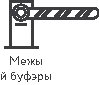
\includegraphics[scale=1.5]{willpower/ch7/5.pdf}
\end{figure}

\emph{Згадайце, як у~фільме «Зьзяньне» герой Джэка Нікалсана бесьперапынна набіраў на друкарцы фразу ``All work and no play makes Jack a dull boy'' (Пастаянная праца без забаваў робіць Джэка нудным хлопцам).}

\subsection*{Усталёўвайце прыярытэты}

Прэфрантальная кара працуе лепш, калі ў~нас выразна зададзеныя прыярытэты, інакш любая ўваходная інфармацыя будзе мець для мозгу аднолькавую важнасьць. Чым лепш мы бачым свае мэты, тым менш адцягваемся, застаёмся ўстойлівейшымі да стрэсаў і лепш працуем.

\emph{Перад працай выразна пагаварыце пра сябе, чым канкрэтна вы зьбіраецеся займацца: ``Што я зараз буду рабіць і навошта?'' Калі цяжка сказаць адразу, дык варта засяродзіцца і сфармуляваць.}

\begin{figure}[htb!]
  \centering
  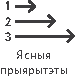
\includegraphics[scale=1.5]{willpower/ch7/6.pdf}
\end{figure}

Вельмі важна мець у~жыцьці вялікія мэты і ясныя прыярытэты, бо нашая стрэсавая сыстэма калібруецца ў~залежнасьці ад выстаўленых задач. Калі ў~вас у~жыцьці ёсьць вялізная важная задача, то ў~параўнаньні зь ёю значнасьць бытавых стрэсаў цьмянее, і яны не здаюцца сур'ёзнымі. Калі такіх мэтаў няма, то нават дробязі будуць лёгка чапляць і выводзіць зь сябе.

\subsection*{Ліквідуйце лішняе}

Як той казаў, «мудрасьць у~тым, каб выдаліць са свайго жыцьця ўсё няважнае». Вельмі часта перагрузка і стрэс узьнікаюць, калі мы бяром на сябе занадта шмат непатрэбных справаў і абавязкаў. Іх дэлегаваньне~--- важная частка антыстрэсавага рэжыму. У ідэале мы павінны займацца тым, што ніхто акрамя нас у~дадзенай сытуацыі ня можа зрабіць, ці тым, што найлепш атрымліваецца менавіта ў~нас. Часьцей пытайцеся ў~сябе: «А ці тым я займаюся?» Амаль усё вакол нас~--- гэта шум, карысных справаў шмат, а~факусавацца важна на самых каштоўных для нас.

\textbf{Ахоўнае тармажэньне}~--- гэта нэрвовы працэс, які складаецца ў~прыгнёце або апярэджаньні іншай хвалі ўзбуджэньня. Ахоўнае тармажэньне дапамагае нам спыняць думаць пра што-небудзь, закрываць працэсы. Скажыце сабе, што гэта няважна, нецікава, непатрэбна. Вельмі часта мы працягваем рабіць нешта па інэрцыі, і потым нам становіцца шкада вытрачаных намаганьняў. Пазбаўляйцеся ад лішняга.

\subsection*{Разгружайце мозг}

Не трымайце ў~ім розныя ідэі, думкі і пляны~--- няхай пад рукой заўсёды будзе нататнік, куды можна ўсё занатаваць. Таксама ў~канцы дня вы можаце выпісваць усе думкі, якія толькі прыходзяць вам у~галаву, гэта выдатна памяншае стрэс. Прааналізуйце сваё працоўнае месца~--- што адцягвае вас? Спрасьціце свой дзень~--- выдаляйце ўсё, што замінае прадуктыўнасьці, максімальна палягчайце рутыну. Майце выразны алгарытм працы з~уваходнай інфармацыяй, не дазваляйце яе плыні перагружаць вас. 

\begin{figure}[htb!]
  \centering
  
\includegraphics[scale=1.5]{willpower/ch7/7.pdf}
\end{figure}

\infobox{Выбірайце ў~моманце: альбо запісаць і адкласьці, альбо зрабіць проста зараз,~--- але не трымайце інфармацыю ў~галаве.}

\subsection*{Ужывайце аўтаматызацыю}

Зьвядзіце да мінімуму колькасьць рашэньняў, якія прымаюцца штодня, бо нават выбар адзеньня можа забраць у~вас прыкметную колькасьць кагнітыўнай энэргіі. 

\emph{Можна выкарыстоўваць наборы гатовых рашэньняў: камплекты адзеньня, мэню на дзень і на тыдзень, гатовыя чэк-сьпісы і сьпісы для розных сытуацыяў.}

\subsection*{Купляйце сабе час}

Дасьледаваньні паказваюць, што час можна купіць: гэта наём людзей пасядзець зь дзецьмі, прыбраць хату, пакасіць траву, ажно да асабістага памочніка. І вытраты на куплю часу робяць людзей нашмат больш шчасьлівымі, чым на куплю матэрыяльных дабротаў. Падумайце, якую працу вы можаце дэлегаваць іншым людзям, як расчысьціць сабе больш часу?

\subsection*{Вучыцеся гаварыць «не»}

Мы хочам падабацца іншым людзям, таму нам хочацца згаджацца з~імі~--- так задумана эвалюцыяй. Ветлівая адмова~--- гэта просты спосаб разгрузіць сябе. Навучыцеся адмаўляць, дазваляючы чалавеку захаваць твар. Трэніруйцеся супрацьстаяць грамадскай думцы і ня бойцеся расчараваць іншых. Заўсёды бярыце паўзу, каб абдумаць любую прапанову, ніколі не згаджайцеся адразу.

\begin{figure}[htb!]
  \centering
  
\includegraphics[scale=1.5]{willpower/ch7/8.pdf}
\end{figure}

\subsection*{Пераключайцеся}

Пераключэньне паміж рознымі аспэктамі працы дапамагае адпачыць без адпачынку, бо за розныя аспэкты справаў адказваюць розныя нэўронавыя контуры. Напрыклад, вы можаце чаргаваць рутуну і навізну, працу з~камандай і аўтаномнасьць, задачы~--- ад тых, дзе канцэнтрацыя не патрабуецца, да тых, якія займаюць максімум увагі.

\begin{figure}[htb!]
  \centering
  
\includegraphics[scale=1.5]{willpower/ch7/9.pdf}
\end{figure}

\subsection*{Балянс рытуал--манатоннасьць}

З аднаго боку, наш мозг любіць рытуалы, таму так эфэктыўна рабіць адно і тое ж у~адзін і той жа час, выкарыстоўваць рытуалы для падрыхтоўкі да працы, адпачываць з~дапамогай аднастайных паўтаральных дзеяньняў. Але зь іншага боку, важна пазьбягаць манатоннасьці, якая вядзе да зьніжэньня ўзроўню гармону актыўнасьці арэксіну. Мае сэнс кожны дзень рабіць нешта ўнікальнае, уносіць элемэнты навізны: спрабуйце сядзець на розных месцах, хадзіць рознымі маршрутамі, выкарыстоўваць розныя крыніцы інфармацыі.

\subsection*{Курс на аднаўленьне}

У спорце існуе яснае разуменьне таго, што фізычныя нагрузкі без аднаўленьня небясьпечныя зьніжэньнем вынікаў. Адэкватнае аднаўленьне~--- ключ да росту. Дакладна гэтак жа і ў~стрэсе~--- важна новую нагрузку браць не адразу пасьля папярэдняй, а~ў пункце супэркампэнсацыі, калі энэргія ўжо аднавілася.

\begin{figure}[htb!]
  \centering
  
\includegraphics[scale=1.5]{willpower/ch7/10.pdf}
\end{figure}

\infobox{Фізычная актыўнасьць, час сярод блізкіх людзей~--- гэта выдатныя спосабы завяршыць стрэс і ўключыць рэжым аднаўленьня.}

Антыстрэсавы лад жыцьця мяркуе, што большую частку дня мы арганізуем як адпачынак, вылучаем ня больш за 4--6 гадзінаў на максімальнае засяроджваньне, а~астатні час~--- на нізкастрэсавыя заняткі. Гэта дапамагае нам быць супэрпрадуктыўнымі, замест таго каб па 10 гадзінаў хаатычна пераключацца паміж рознымі справамі. Вылучайце хаця б адзін дзень нау тыдзень на якасны адпачынак у~выглядзе розных абмежаваньняў: бяз працы, без смартфона, на інфармацыйнай і дафамінавай дыеце, прысьвяціўшы яго адпачынку і разважаньням.

\emph{Фрамінгемскае дасьледаваньне сэрца вызначыла сувязь паміж адпачынкамі і сардэчна-сасудзістымі захворваньнямі: адпачынак менш за тры тыдні на год прыводзіў да павелічэньня сьмяротнасьці на 37\,\%. Нічога дзіўна ў~гэтым няма, іншыя дасьледаваньні таксама пацьвярджаюць гэтыя назіраньні. Вучыцеся адпачываць эфэктыўна. Вось некалькі ідэяў для якаснага адпачынку.}

\textbf{Папераджальны адпачынак супроць канчатковага.} Чым раней вы пачалі адпачываць і рабіць перапынкі, тым даўжэй прапрацуеце безь зьнясіленьня. Ідэя «адпачываць толькі як усё скончу» заганная. Паўзы~--- гэта не марнаваньне часу, а~«заточваньне касы». Падтрымлівайце ваш мозг у~добрым стане, не перагружайце яго.

\textbf{Заплянаваны адпачынак супроць «які натрапіцца».} Ідэальны адпачынак~--- гэта той, які вы загадзя заплянавалі. Паспрабуйце ў~штотыднёвік першымі ўносіць рэкрэацыйныя актыўнасьці, расьпішыце, дзе і як вы будзеце адпачываць, час для хобі і прыемных справаў. А ўжо на рэшту часу~--- працу. Прадчуваньне адпачынку~--- ужо адпачынак і стрэсаўстойлівасьць сёньня.

\textbf{Зьмена кантэксту супроць манатоннасьці.} Адпачываць і працаваць за адным сталом~--- гэта кепская ідэя. Выкарыстоўвайце розны кантэкст для розных актыўнасьцяў. Таму паехаць некуды, дзе няма ніякіх асацыяцыяў з~працай ці звыклымі клопатамі, эфэктыўна разгружае.

\textbf{Чысты адпачынак супроць паўработы.} Спрабаваць памяншаць нагрузку на сябе, даваць працоўныя патураньні ці зьмяншаць тэмп ня вельмі карысна. Лепш перапыніцца і аднавіць свой узровень энэргіі. А пачынаючы працаваць~--- забясьпечыць сабе глыбокае занурэньне.

\textbf{Спантаннасьць супроць «як звычайна».} Спантаннасьць, выпадковасьць, навізна заўсёды асьвяжаюць і бадзёраць. Кіньце жэрабя, куды пайсьці, тыцніце пальцам у~мапу і пабывайце ў~гэтым месцы. Любое адступленьне ад рутыны выдатна перазагружае. Крэатыўнасьць, лёгкая вар'яцінка добра балянсуе стомленую прэфранталку.

\textbf{Актыўны адпачынак супроць пасіўнага.} Пасіўны адпачынак накшталт ляжаньня на канапе ці зразаньне вуглоў да дафаміну (выпіць, заесьці, сэрфіць) не такі эфэктыўны. Актыўны адпачынак вучыць вас атрымліваць дафамін больш складанымі, але больш эфэктыўнымі шляхамі. Схадзіць на танцы, згуляць у~тэніс, пашпацыраваць у~восеньскім парку.

\textbf{Пераўтваральны адпачынак супроць спажывальнага.} Адпачынак, калі мы проста пасіўна спажываем нешта, не такі эфэктыўны, як пераўтваральны адпачынак. Напрыклад, нават мэдыя можа валодаць эфэктам катарсісу, стымулюючы нас прарабіць унутраную працу. Творчасьць стымулюе ствараць новае, зьмяняць існае. Мы ня проста вяртаемся да сябе ранейшых, а~ўзьнімаемся вышэй над сабой.

\subsection*{Пытаньні і заданьні}

1. Якія самыя раньнія прыкметы стомы вы ў~сабе заўважаеце?

2. Ці надаяце вы ўвагу плянаваньню сваёй працы і падтрымцы працаздольнасьці?

3. Чатыры кіты рэжыму: харчаваньне, рух, сон і праца. Ці атрымліваецца ў~вас іх сынхранізаваць і падтрымліваць?


\section{Добры стрэс}

«Стрэс~--- гэта водар і смак жыцьця»,~--- казаў Ганс Сэлье, заснавальнік вучэньня аб стрэсе. Сама энэргія стрэсу~--- бяз знакаў «плюс» або «мінус», стрэс як полымя~--- можа сагрэць, на ім можна гатаваць, але яно ж можа і пакінуць глыбокія апёкі. 

\begin{figure*}[htb!]
  \centering
  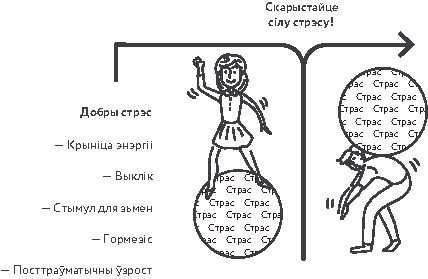
\includegraphics[scale=1.5]{willpower/ch7/11.pdf}
\end{figure*}

\textbf{Ня ўсякі стрэс~--- гэта шкодна, карысны стрэс мае асобную назву~--- эўстрэс.} Ён забясьпечвае нас энэргіяй, павялічвае матывацыю і ўстойлівасьць. 

\emph{Дасьледаваньні паказваюць, што паміж колькасьцю стрэсу і здароўем існуе U-падобная залежнасьць: малая і вялікая колькасьць стрэсу зьвязаная з~горшым здароўем, а~вось сярэдняя колькасьць стрэсу карысная. Людзі, якія перажылі шэраг небясьпечных сытуацыяў, шчасьлівейшыя, чым тыя, хто цалкам патрапляў пазьбегнуць стрэсавых сытуацый.}

\textbf{Карысны стрэс}~--- гэта кароткі і кіраваны стрэс, з~магчымасьцю адэкватнага аднаўленьня. Асоба добры фізычны стрэс, на дэфіцыт якога мы пакутуем: гэта халодныя абліваньні, умераныя трэніроўкі.

Псыхалягічны гостры стрэс таксама можа быць карысны як каталізатар зьменаў. Калі цела і псыхіка адаптуюцца да нагрузкі, мы становімся мацнейшымі, а~досьвед пераадоленьня стрэсавых сытуацыяў аказваецца карысны ў~будучыні. Ганс Сэлье лічыў, што пазьбягаць трэба ня стрэсу, а~зьнясіленьня ад яго.

Разглядаючы стрэс як сябра, мы ня толькі зьмяншаем шкоду ад яго, але й можам атрымліваць карысьць, ператвараючы перашкоды ў~сродкі дасягненьня мэты. Калі няма напругі, дык робіцца нудна: кароткі стрэс павялічвае навучаньне і засваеньне новага, дапамагае нам хутчэй прымаць зьмены. Энэргія стрэсу~--- як хваля, на якой вы можаце пракаціцца і сілу якой можаце выкарыстоўваць. Любоў да зьменаў~--- гэта смак да жыцьця. Дасьледаваньні паказалі, што тыя, хто перажыў шэраг небясьпечных сытуацыяў, больш шчасьлівыя за тых, хто цалкам патрапляў пазьбегнуць стрэсавых сытуацыяў.

\subsection*{Успрыманьне стрэсу і ягонае шкоды}

Калі мы ўспрымаем стрэс як шкодны фактар, гэта можа спрацаваць як нацэба (антыплацэба): перабольшаньне яго небясьпекі і неспакой з~гэтай нагоды павялічвае рэальныя рызыкі для здароўя. Зьмяніўшы сваё стаўленьне, мы зьменім і свае рэакцыі, зьнізіўшы нэгатыўнае ўзьдзеяньне стрэсу.

\emph{У адным з~дасьледаваньняў паддосьледных ставілі пад псыхалягічны стрэс, прымушаючы выступаць і вырашаць задачы, у~працэсе крытыкуючы іх, абрываючы, лаючы за памылкі. Але адной групе патлумачылі: стрэс не нясе пагрозы, а~дапамагае мабілізаваць рэсурсы, увагу і энэргію, пачашчэньне пульсу~--- гэта больш кіслароду, цяглічны тонус~--- гатоўнасьць змагацца і да т.~п. Падрыхтаваныя ўдзельнікі паказалі лепшыя вынікі, хутчэй аднавіліся, а~самае галоўнае~--- давалі іншую фізыялягічную рэакцыю: пры павышэньні пульсу ў~іх назіралася расслабленьне сасудаў, а~не звужэньне, як у~кантрольнай групе. Такая рэакцыя зьніжае рызыку сардэчна-сасудзістых захворваньняў.}

Калі мы сфакусаваныя на нэгатыўных чаканьнях, гэта можа адыграць ролю «самавыканальнага прароцтва», калі нашыя чаканьні вядуць да неадаптыўнай рэакцыі і пераконваюць нас у~праўдзівасьці нашых уяўленьняў («а я казаў»).

\subsection*{Стрэс і перабудова нэўронавых сувязяў}

«Для посьпеху ў~жыцьці патрэбныя сувязі, моцныя нэўронныя сувязі»,~--- жартуюць нэўрафізыёлягіі. Але насамрэч нам патрэбныя гнуткія нэўронныя сувязі, бо нам трэба не вучыцца, а~перавучвацца. 

\emph{На гэта асабліва зважаў амэрыканскі футуроляг Элвін Тофлер: «Непісьменнымі ў~XXI стагодзьдзі будуць лічыцца ня тыя, хто ня ўмее чытаць і пісаць, а~тыя, хто ня ўмее вучыцца, развучвацца і перавучвацца». Так, для многіх японскіх фірмаў характэрная ратацыя і перавучваньне пэрсаналу новым спэцыяльнасьцям кожныя 3--5 гадоў.}

Перавучвацца нашмат складаней, чым проста вучыцца новаму. Рэч у~тым, што пры доўгім занятку адным і тым жа нэўронныя сувязі, якія кіруюць гэтым працэсам, становяцца досыць трывалымі. Гучыць быццам бы добра? Насамрэч гэта ня так. Устаноўлена, што здольны на больш эфэктыўнае навучаньне мозг валодае гнуткасьцю і здольнасьцю адразу перабудоўваць злучэньні з~мэтай засваеньня новых ведаў~--- гэта называецца высокая нэўраплястычнасьць. Залішняя «калянасьць» нэўронавых шляхоў зьвязаная з~горшай навучальнасьцю.

Як вядома, стрэс выклікае зьніжэньне колькасьці нэрвовых сувязяў (бяз гібелі нэўронаў)~--- вось гэта гучыць ня вельмі.

\textbf{Часам менавіта зьніжэньне колькасьці нэрвовых сувязяў зьяўляецца дабрадайнай глебай для зьменаў, бо яно вядзе да фармаваньня «вольнага поля».} Памятаеце ўсходнія фільмы, дзе стары мудры настаўнік укідвае вучня ў~стан стрэсу і толькі потым пачынае навучаньне? Чаму ён гэта робіць? Мэта~--- выкарыстаньне стрэсу для аслабленьня звыклай хваткі звычак і стварэньня «поля для зьменаў». Сапраўды, значныя зьмены асобы рэдка адбываюцца самі па сабе, як правіла, іх крыніцай зьяўляецца сур'ёзны стрэс.

Гэты фэномэн атрымаў назву «посттраўматычнага росту», калі ў~чалавека адбываецца пераацэнка каштоўнасьцяў, усьведамленьне каштоўнасьці жыцьця ў~цэлым, узьнікае «гатоўнасьць да дзеяньняў», выяўляюцца новыя магчымасьці і па-іншаму ацэньваюцца асабістыя якасьці. 

\infobox{Калі мы захоўваем кантроль, пачуцьцё ўласнае вартасьці і эфэктыўнасьць, імкненьне знайсьці асэнсаваную мэту ў~жыцьці, пазітыўныя эмоцыі і пачуцьцё гумару, падтрымку блізкіх, то нам нашмат лягчэй атрымаць карысьць ад стрэсу.}

\emph{Некаторыя навукоўцы нават вылучылі канцэпцыю «другога нараджэньня» аб тым, што для радыкальных зьменаў у~жыцьці, для разьвіцьця лідэраў неабходнае ўзьдзеяньне траўмавальных падзей, якія зьмяняюць погляды, якія прыводзяць да азарэньня і пераасэнсаваньня.}

\subsection*{Экспазыцыйная тэрапія}

Некаторыя людзі лічаць, што можна зьменшыць стрэс, проста ўцякаючы або ўхіляючы яго крыніцы. Маўляў, няма стрэсу~--- няма праблемаў. Але, на жаль, гэта не працуе. Калі мы будзем пазьбягаць стрэсараў, то наша адчувальнасьць да стрэсу толькі вырасьце. 

\textbf{Чым часьцей мы робім тое, што выклікае ў~нас стрэс, тым менш гэта нас траўмуе.} Будысты і стоікі з~даўніх часоў выкарыстоўвалі нэгатыўную візуалізацыю, пражываючы гора і няшчасьці, якія зь імі адбываліся.

Уяўляючы разьвіцьцё сцэнароў па найгоршым варыянце, мы ўсьведамляем, што нават у~гэтым выпадку зможам знайсьці сілы жыць далей і даць рады са стрэсам. Заадно гэта дапаможа атрымліваць больш задавальненьня ад жыцьця~--- уявіце, што вы пазбавіліся ўсяго. А сутыкнуўшыся са стрэсам, уявіце і пражывіце яшчэ горшыя варыянты разьвіцьця падзеяў~--- гэта дапаможа зразумець, што цяпер ня ўсё так кепска. 

\emph{Стрэс-прышчэпкавая тэрапія~--- гэта дазаванае даданьне стрэсу, калі мы вучымся трываць нагрузку.}

\subsection*{Гармэзіс, або «Тое, што не забівае, робіць нас мацнейшымі»}

Для нашага цела карысным зьяўляецца і дазаванае ўзьдзеяньне розных шкодных чыньнікаў. Яны стымулююць ахоўныя сілы і аднаўленьне арганізма, паляпшаюць здароўе. Да іх адносяцца фізычныя трэніроўкі, харчовыя абмежаваньні (фастынг і галаданьні), холад (розныя віды гартаваньня), цеплавыя чыньнікі (саўна), зьмена ўтрыманьня кіслароду (гіпаксічныя трэніроўкі або гіпэрбарычная аксігенацыя, гіпаксія на трэніроўцы, ныраньне, уздым у~горы), узьдзеяньне на цела (іголкаўколваньне, масаж, нават драпіна і сіняк) і нават іянізавальная радыяцыя.

\emph{Як ні парадаксальна, але высьветлілася, што работнікі атамных станцый маюць у~два разы меншую рызыку раку. З тэрапэўтычнымі мэтамі выкарыстоўваюцца радонавыя ванны.}

Некаторыя злучэньні ў~прадуктах харчаваньня, такія як поліфэнолы, таксама стымулююць гармэзіс~--- і гэта ўжо будзе фітанутрыентны стрэс: напрыклад, кафэін у~расьлінах працуе як яд для абароны ад казюрак, але гэты аб'ём «яду» ўзьдзейнічае на чалавека падбадзёрліва. Або сілімарын~--- рэчыва ў~пладах растаропшы~--- уплывае на печань чалавека і зьяўляецца гепатапратэктарам.

\subsection*{Пытаньні і заданьні}

1. У якіх выпадках стрэс і нагрузка надаюць вам сілы і натхняюць?

2. Ці былі ў~вашым жыцьці такія сытуацыі, калі стрэс мяняў вашыя погляды і прымушаў пераасэнсаваць каштоўнасьці?

3. Якія крыніцы карыснага стрэсу ёсьць у~вашым жыцьці? Што яшчэ можна дадаць?


\section{Псыхалягічныя рэсурсы стрэсаўстойлівасьці}

Псыхалягічныя навыкі стрэсаўстойлівасьці~--- гэта наш «софт»: чым гэтыя праграмы лепш у~нас прапісаныя, тым аптымальней мы спраўляемся са стрэсам, не пакутуем ад яго, а~разьвіваемся зь ім. Мы ж не расьліны, не гародніна, якія прывязаны да зямлі, мы здольныя адаптавацца і мяняцца.

\subsection*{Мозг ня бачылі?}

Часта дзеяньне моцнага стрэсара прыводзіць да аўтаматычнай рэакцыі, калі мігдаліна літаральна «крадзе мозг», і чалавек губляе кантроль над сабой, выбухае.

\emph{Кажуць, у~цара Саламона таксама была праблема «крадзежу мозгу», калі ён літаральна закіпаў ад лютасьці. Яму дапамог пярсьцёнак з~фразай «Усё мінае». Досыць было пары сэкундаў, каб адцягнуцца і прачытаць надпіс, як імпульс цішэў. Аднойчы гэта не дапамагло, і ён сарваў пярсьцёнак… Але спрацаваў надпіс на ўнутраным баку: «І гэта міне».}

Сэнсарная інфармацыя ўваходзіць у~мозг, праходзіць праз таламус і далей ёсьць два шляхі: яна можа ісьці па «кароткім», актывуючы амігдалу (бі або бяжы), і па «доўгім»~--- праз прэфранталку (падумай, а~потым рабі). У старажытнасьці кароткі хуткі шлях рэагаваньня дапамагаў нам выжыць пры нападзе драпежніка, але цяпер ён трымае нас у~аброці страху і аўтаматызму. Свабода ад аўтаматычных рэакцый нараджаецца ў~прэфрантальнай кары~--- тут жыве навык вытрымліваць паўзу між стымулам і рэакцыяй. Бяз гэтага навыку мы вырачаныя паўтараць «дзень байбака».

\emph{Як пісаў псыхоляг Віктар Франкл: «Паміж стымулам і рэакцыяй ёсьць прамежак. У гэтым прамежку мы маем свабоду выбару сваёй рэакцыі. Ад гэтага выбару залежыць нашае разьвіцьцё і шчасьце».}

\subsection*{Ацэнка стрэсара}

Для таго каб абраць правільную рэакцыю, неабходна адэкватна ацэньваць стрэсар. У гэтым дапаможа паўза: усяго 4 сэкунды, удых і выдых, і гэтага будзе дастаткова, каб прэфрантальная кара ўключылася ў~ацэнку сытуацыі. Не хвалюйцеся, што будзеце выглядаць недарэчна, хутчэй наадварот~--- такая марудлівасьць створыць вам імідж чалавека, які адказвае за свае словы. І нават калі стрэс непазьбежны, правільнае яго выкарыстаньне ператворыць энэргію стрэсу ў~натхненьне і выклік, а~не ў~трывогу. Далей, уласна, ацэнка: пагрозу нясе стрэс ці сама стрэсавая рэакцыя, ці патрэбныя дадатковыя ахоўныя меры? Вы ж памятаеце, што самым шкодным зьяўляецца некантраляваны стрэс, дык што ж вы можаце адразу ўзяць пад кантроль?

\begin{figure}[htb!]
  \centering
  
\includegraphics[scale=1.5]{willpower/ch7/12.pdf}
\end{figure}

Наш мозг перадуім ацэньвае стрэсар праз прызму нашай асобы, ці зьяўляецца стрэсар значным, спрыяльным або небясьпечным? Калі стрэсар небясьпечны, то ідзе ацэнка наяўных у~нас рэсурсаў. Калі рэсурсаў стае, мы спакойна рашаем пытаньне. Калі рэсурсаў бракуе, то падключаюцца копінг-стратэгіі, калі мы можам зьмяніць саму сытуацыю або зьмяніць сваю эмацыйную рэакцыю на сытуацыю.

Калі рэсурсаў у~нас мала, то мозг уключае псыхалягічныя абароны, пры якіх чалавек як быццам ізалюецца ад праблемы, не ўсьведамляе пагрозы, мае скажонае ўспрыманьне рэчаіснасьці. А вось копінг дазваляе больш мэтанакіравана падысьці да сытуацыі, якую мы ня можам вырашыць. Абавязкова перабярыце некалькі варыянтаў: калі ў~вас толькі адна ідэя, што рабіць, дык гэта ня вельмі добра. Пачынайце дзейнічаць, толькі калі ў~вас ёсьць мінімум тры розныя варыянты рашэньня пэўнай праблемы.

Варыянты: 
\begin{itemize}
  \item \textbf{ліквідаваць стрэсар}: прыняць меры для вырашэньня праблемы, адысьці ад праблемы;
  \item \textbf{зьнізіць узровень стрэсу}: адаптаваць сваю фізыялягічную рэакцыю;
  \item \textbf{зьмяніць сваё стаўленьне да стрэсара}: зьнізіць важнасьць стрэсара;
  \item \textbf{зьмяніць свае паводзіны}: выбраць іншую копінг-стратэгію.
\end{itemize}

\emph{Для таго каб сытуацыя стала стрэсавай, яна павінна зьмяшчаць адзін з~чыньнікаў N.U.T.S.: навізна (Novelty), непрадказальнасьць (Unpredictability), ацэнка пагрозы (Threat per\-cep\-tion), пачуцьцё страты кантролю (Sense of no control). Антыстрэс-канцэпцыяй будзе праца з~кожным з~гэтых чыньнікаў.}

\textbf{Ацаніце сваю рэакцыю}: ці прапарцыйны ваш адказ стрэсу, ці ведаеце вы, калі выключыць стрэсавую рэакцыю і як яе абмежаваць у~часе? Падумайце, як пераразьмеркаваць рэсурсы для вырашэньня ўзьніклай праблемы, што вам трэба адпусьціць, а~якія рэсурсы можна выкарыстоўваць у~гэтай сытуацыі. Калі нешта ўжо страчана, дык, магчыма, ужо ня варта за гэта і змагацца, крыўдаваць ці шкадаваць?

\textbf{Копінг-стратэгіі} (ад англ. to cope with~--- даваць рады, спраўляцца)~--- гэта праграмы, якіх прытрымліваецца чалавек, каб даць рады стрэсу. Яны могуць быць карыснымі ў~адным выпадку і шкоднымі ў~іншым. Выбар правільнай стратэгіі~--- важнае рашэньне, якое падвышае стрэсаўстойлівасьць. Можна дзейнічаць у~адзіночку ці сацыяльна, можна актыўна вырашаць праблему альбо ўхіляцца ад яе, можна дзейнічаць актыўна ці пасіўна.

\begin{figure}[htb!]
  \centering
  
\includegraphics[scale=1.5]{willpower/ch7/13.pdf}
\end{figure}

Тыповымі копінг-стратэгіямі зьяўляюцца:
\begin{enumerate}
  \item \textbf{Канфрантацыя}~--- актыўнае вырашэньне праблемы, адстойваньне сваіх інтарэсаў у~канкрэтных дзеяньнях, можа быць не заўсёды адаптыўнай.
  \item \textbf{Дыстанцыяваньне}~--- зьніжэньне значнасьці праблемы, зьніжэньне эмацыйнай уцягнутасьці, абясцэньваньне стрэсара, пераключэньне ўвагі і да т.~п. У некаторых сытуацыях карысным будзе «рэпрэсіўны копінг», калі людзі схільныя пазьбягаць нэгатыўных думак, эмоцыяў і ўспамінаў.
  \item \textbf{Самакантроль}~--- пераадоленьне праблемы за кошт стрымліваньня эмоцыяў і мэтанакіраваных паводзінаў, высокае самавалоданьне.
  \item \textbf{Пошук падтрымкі}~--- прыцягненьне вонкавых рэсурсаў, звычайна людзей, чаканьне дапамогі, парады, увагі.
  \item \textbf{Прыняцьце адказнасьці}~--- прызнаньне сваёй адказнасьці за праблему, часта з~элемэнтамі віны і самакрытыкі, можа спалучацца з~хранічнай незадаволенасьцю сабой.
  \item \textbf{Уцёкі-пазьбяганьне}~--- ухіленьне ад вырашэньня праблемы за кошт яе адмаўленьня, фантазіі або рэгрэсіі. У некаторых катастрафічных выпадках адмаўленьне можа быць найлепшай стратэгіяй, каб захоўваць надзею.
  \item \textbf{Плянаваньне}~--- аналіз сытуацыі і выпрацоўка рацыянальнай стратэгіі яе вырашэньня.
  \item \textbf{Станоўчая пераацэнка}~--- пераасэнсаваньне праблемы як стымулу для асобаснага росту, знаходжаньне ў~ёй станоўчых момантаў.
\end{enumerate}

Дадатковыя чыньнікі стрэсаўстойлівасьці ўключаюць давер і шчаснае сацыяльнае асяродзьдзе, каапэрацыю з~іншымі людзьмі і, як ні парадаксальна, пэўнае самаўзвышэньне: лічыцца, што прымаць свае абмежаваньні карысна, але часам завышаная самаацэнка і нерэалістычныя перадузятасьці адносна сябе спрыяюць дабрабыту і павышаюць устойлівасьць перад стрэсам.

\subsection*{Пытаньні і заданьні}

1. Ці ўмееце вы зрабіць паўзу перад рэакцыяй на стрэсар?

2. Якія чыньнікі робяць сытуацыю стрэсавай? Як зь імі можна справіцца?

3. Якімі копінг-стратэгіямі часьцей за ўсё вы карыстаецеся? Ці эфэктыўныя, ці адэкватныя яны?


\section{Жыцьцеўстойлівасьць}

Калі копінг-стратэгіі~--- гэта, хутчэй, альгарытмы дзеяньня, то жыцьцеўстойлівасьць~--- гэта ўласьцівасьць асобы, самы важны псыхалягічны рэсурс стрэсаўстойлівасьці. Жыцьцеўстойлівасьць~--- гэта цэлая сыстэма перакананьняў пра сябе, сьвет і адносіны зь ім, гэта сапраўдная «мужнасьць быць» у~рэальным сьвеце. З пункту гледжаньня нашае цьвёрдасьці і сілы супрацьдзеяньня мы~--- гэта тое, як мы змагаемся. Людзі з~высокай жыцьцеўстойлівасьцю менш хварэюць і маюць лепшае здароўе незалежна ад узроўню стрэсу і нават у~адсутнасьці сацыяльнай падтрымкі. Жыцьцеўстойлівасьць узмацняе ўзровень шчасьця і ўпэўненасьці ў~сабе, дапамагае чалавеку вытрымліваць стрэсавую сытуацыю, захоўваючы пры гэтым унутраны балянс і гармонію, палягчае адэкватнае бачаньне сытуацыі, прызнаньне сваіх рэальных магчымасьцяў і сваёй уразьлівасьці. Менавіта гэта, у~сваю чаргу, дапамагае трансфармаваць нэгатыўныя ўражаньні ў~новыя магчымасьці і «рабіць ліманад зь лімонаў». Калі ж мы мінаем небясьпечныя сытуацыі, то падобная мяккасьць паступова разбурае нашу стрэсасутаўстойлівасьць.

\emph{Такі тып людзей, якія ўхіляюцца, мае горш разьвітую ўсьвядомленасьць, самаідэнтыфікацыю, яны ня могуць адэкватна ацэньваць сытуацыі і лічаць сябе няздольнымі кантраляваць тое, што адбываецца зь імі. Мяккія людзі пазьбягаюць стрэсаў або «цярпяць» іх, часта пэсімістычна настроеныя, маюць нізкую матывацыю і сыходзяць у~ілюзіі замест рашэньня праблемаў.}

\infobox{Давайце разьбяромся, зь якіх ключавых кампанэнтаў складаецца разьвіцьцё жыцьцеўстойлівасьці.}

\subsection*{Уключанасьць}. Уключанасьць~--- гэта перакананасьць у тым, што вялікая ўцягнутасьць ва ўсё, што адбываецца навокал, дае й вялікія шанцы знайсьці нешта цікавае і важнае для сябе асабіста. Гэта адчуваньне ўдзелу ў~плыні жыцьця, поўнае ўключэньне ў~вырашэньне жыцьцёвых задач, разуменьне таго, што я магу прымаць ва ўсім удзел і ўплываць на тое, што адбываецца. 

\begin{figure}[htb!]
  \centering
  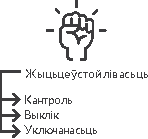
\includegraphics[scale=1.5]{willpower/ch7/14.pdf}
\end{figure}

\infobox{Калі мы ўключаныя ў~жыцьцё, то мы поўнасьцю аддаёмся сваёй справе, падзяляем яе сэнсы і мэты, прымаем на сябе абавязкі да выкананьня.}

Наша асоба як бы зьліваецца з~намерам выканаць справу і дасягнуць выніку, з~адчуваньнем, што ўсё магчыма, што мы здольныя рэалізаваць сябе, і гэта, вядома, дае адчуваньне ўласнай каштоўнасьці. Таму асьцерагайцеся тых людзей, якія маніпуляцыямі выклікаюць думкі, што «ад вас нічога не залежыць, ня трэба нават спрабаваць». Калі мы ўключаныя, сьвет для нас не абыякавы, і мы матываваныя на актыўнасьць.

\emph{Выключанасьць, ці адчужэньне ад таго, што адбываецца, узмацняе адчувальнасьць да стрэсу і прыносіць адчуваньне, што жыцьцё праходзіць міма. Актыўна прымайце ўдзел ва ўсіх аспэктах жыцьця: схадзіць на мітынг, паўдзельнічаць у~сходах груп, арганізаваць якую-небудзь справу, уключыўшыся ў~жыцьцё свайго пад'езда, школы, калектыву, і далей пашыраючы зону ўплыву. Цікаўцеся тым, што адбываецца вакол вас, і вырашайце заўважаныя праблемы. Пазыцыя «мая хата з~краю» небясьпечная для здароўя.}

\subsection*{Кантроль} 

Унутраны локус кантролю~--- гэта ўпэўненасьць (аб'ектыўная або суб'ектыўная) у~тым, што мы можам уплываць на хаду падзей, што мы здольныя дамінаваць над абставінамі, зьмяніць усё ў~лепшы бок, пасьпяхова супрацьстаяць нават самым цяжкім момантам жыцьця. Калі нас пазбавіць кантролю, гэта выклікае адчуваньне бездапаможнасьці і павялічвае нэгатыўнае дзеяньне стрэсу. Некантраляваны стрэс часта выкарыстоўваецца як маніпулятарная тэхніка для павышэньня кіравальнасьці ў~школах, войсках, сэктах ды іншых гіерархічных калектывах, дзе пачаткоўцаў выпрабоўваюць.

\emph{Экспэрымэнты амэрыканскага псыхоляга Марціна Сэлігмана паказалі, што працяглы некантраляваны стрэс вядзе да фарміраваньня вывучанай бездапаможнасьці, калі жывёлы і людзі адмаўляюцца нат спрабаваць нешта зьмяніць нават у~спрыяльных абставінах. Гэта прыводзіць да пасіўнасьці, нежаданьня штосьці зьмяняць. Вывучаная бездапаможнасьць зьвязаная з~дэпрэсіяй і павелічэньнем рызыкі шматлікіх захворваньняў. Любая магчымасьць кантролю вядзе да таго, што стрэс пераносіцца лягчэй, гэта працуе і ў~людзей, і ў~жывёлаў.}

\textbf{Некантраляваны стрэс} складаецца з~наступных кампанэнтаў: 
\begin{itemize}
  \item немагчымасьць прыстасавацца да ўзьдзеяньня;
  \item немагчымасьць пазьбегнуць узьдзеяньня або пазбавіцца яго;
  \item немагчымасьць прадказаць пачатак і канец узьдзеяньня.
\end{itemize}

Важна: выявіць крыніца некантраляванага стрэсу ў~сваім жыцьці і высьветліць, якая асаблівасьць гэтага стрэсара робіць ягонае дзеяньне некантраляваным. 

\emph{У экспэрымэнтах у~доме састарэлых павелічэньне магчымасьці выбіраць бытавыя аспэкты свайго жыцьця (музыка, ежа, абстаноўка пакояў і да т.~п.) прывялі да прыкметнага паляпшэньня здароўя ва ўдзельнікаў. Калі на людзей узьдзейнічае шум, але ім сказана, што яны могуць пазбавіцца яго па жаданьні, яны трываюць такое ўзьдзеяньне нашмат лягчэй і захоўваюць больш высокую працаздольнасьць.}

На стан уплывае кантроль нават у~паўсядзённых дробязях: напрыклад, самае спакойнае месца ў~перапоўненым ліфце~--- ля панэлі з~кнопкамі. Нават такія моманты могуць павялічыць адчуваньне кіраваньня сваім жыцьцём. Пры гэтым трэба менш увагі надаваць рэчам, якія мы дакладна ня можам кантраляваць. Стаўце сабе мэтай, напрыклад, ня выйграць матч, а~зрабіць усё магчымае, каб яго выйграць,~--- бо ня ўсё залежыць ад вас. Не марнуйце час на шкадаваньне аб мінулым: калі вы спрабуеце паўплываць на тое, што ўжо немагчыма зьмяніць, гэта павялічвае рызыку бездапаможнасьці.

\subsection*{Аўтаномная зона паводзінаў}

Любыя падзеі, якія адбываюцца, дзяліце на «магу кантраляваць» і «не магу кантраляваць», факусуючыся на першых і не марнуючы сілаў на перажываньні аб другіх. Падзяліце ўсе свае дзеяньні на \textbf{рэактыўныя}, якія вы абавязаныя рабіць, і \textbf{праактыўныя}, якія вы можаце рабіць, а~можаце і не рабіць, і нікому ня мусіце справаздачыцца. Павелічэньне колькасьці праактыўных дзеяньняў дабратворна ўплывае на стрэсаўстойлівасьць, бо вельмі важна рабіць хоць нешта, чым не рабіць нічога.

\emph{Нават калі кантроль уяўны, ён усё роўна працуе станоўча. Напрыклад, вы седзіце на доўгай нуднай нарадзе. Цярпець, абурацца, шкадаваць аб страчаным часе~--- найгоршы выбар у~гэтай сытуацыі. Паспрабуйце неўзаметку зьняць абутак і даць нагам адпачыць. У заторы~--- чым рэагаваць лютасьцю, лепей паслухайце музыку ці аўдыёкніжку і зрабіце самамасаж стомленай шыі.}

\textbf{Пошукавая актыўнасьць}~--- гэта любая дзейнасьць, калі мы імкнёмся зьмяніць стрэсавую сытуацыю, нягледзячы на пагрозы і нават пры адсутнасьці гарантыяў посьпеху. Успомніце прыпавесьць пра жабку і збан малака: у~жабкі не было гарантыяў, што яе скачкі дапамогуць, тым ня менш яна не здавалася і выбралася вонкі. Воля да жыцьця, канструктыўная агрэсія і настойлівасьць дапамагаюць у~сытуацыях нават безь відавочнага рашэньня. Будзьце настойлівыя, адкрытыя новаму досьведу, улічвайце і заўважайце нюансы сытуацыі, і гэта можа падказаць вам шлях. 

\infobox{Заўсёды рабіце першы крок: стрэс пачынаецца зь непрыняцьця мераў, а~як толькі вы разумееце, што можаце нешта зрабіць для рашэньня праблемы (даведацца, патэлефанаваць, скласьці плян), стрэс памяншаецца.}

\subsection*{Самастойнасьць і працоўны стрэс}

Адна з~рэчаў, якія я больш за ўсё шаную ў~маёй працы,~--- гэта ступень свабоды ў~выбары таго, што і як трэба рабіць. Працоўная самастойнасьць~--- гэта рэч вельмі карысная для здароўя, яна значна зьніжае ўзровень стрэсу. 

\emph{Дасьледаваньні паказваюць, што пры параўнаньні людзей з~аднолькавым статусам, заробкам і месцам працы, рызыка дэпрэсіі ніжэйшая, калі кантроль над сваёй працай вышэйшы. Таксама ёсьць цалкам выразная залежнасьць паміж рызыкай сардэчна-сасудзістых захворваньняў і працоўнай самастойнасьцю.}

Чым больш вы можаце кантраляваць такія аспэкты свайго працоўнага месца, як кіраваньне сьвятлом, кандыцыянэрам, магчымасьць ставіць фатаграфіі, вешаць асабістыя рэчы, ставіць расьліны, мяняць і перасоўваць мэблю, тым больш гэта карысна для здароўя. 

\textbf{Рэалізацыя сваёй ідэнтычнасьці на працоўным месцы павышае прадуктыўнасьць на 30\,\%.} Павялічвайце сваю магчымасьць кіраваць прасторай, у~якім вы знаходзіцеся. Часьцяком нам шкодзіць ня гэтулькі стрэс, колькі адчуваньне свайго бясьсільля і бездапаможнасьці, немагчымасьці паўплываць на рэчы й падзеі. А калі нізкі кантроль спалучаецца з~падвышанымі патрабаваньнямі і адсутнасьцю падтрымкі, то рызыка для здароўя ўзрастае яшчэ мацней.

\emph{Якая ў~вас ступень працоўнай самастойнасьці? Ці спрабуеце вы яе пашырыць?}

\subsection*{Выклік}

Стрэс~--- гэта асабісты выклік, жыцьцё~--- гэта зьмены, мы мяняемся, пакуль мы жывыя, адаптацыя~--- гэта ключ да разьвіцьця: такое стаўленьне да стрэсу і магчымасьць прымаць жыцьцёвыя выклікі зьяўляецца важным чыньнікам жыцьцяздольнасьці. Калі мы бачым у~стрэсе магчымасьць для разьвіцьця, гэта дазваляе нам заставацца адкрытымі ўсяму, што адбываецца.

\textbf{Рэакцыя «збліжэньня» часьцей за ўсё прадуктыўнейшая за рэакцыю «пазьбяганьня» стрэсара.} Прымаючы выклік, мы гатовы перажыць любы досьвед, і добры, і дрэнны. У кожным выпадку гэта спрыяе разьвіцьцю, бо нават памылка ці пройгрыш даюць нам каштоўную інфармацыю. Боязь прайграць зьбядняе нашае жыцьцё, фанатычнае імкненьне да бясьпекі і камфорту аслабляе нас.

\emph{Падумайце, які выклік можа быць у~вашых стрэсарах? Чаму яны могуць вас навучыць? Разгледзьце і перафармулюйце свае задачы як выклікі, якія вы вітаеце, а~ня цяжар, які імкняцеся пазьбегнуць.}

\subsection*{Самаэфэктыўнасьць}

Гэта ўпэўненасьць у~тым, што мы можам выканаць пэўную працу. Чым больш у~нас практычных навыкаў для выкананьня канкрэтнай дзейнасьці, тым больш мы ў~сабе і ўпэўненыя. Чым вышэй наш досьвед, тым менш напругі мы адчуваем. 

\textbf{Важнай часткай самаэфэктыўнасьці зьяўляецца паняцьце спасьціжэньня~--- то бок перакананасьці, што сьвет вакол нас разумны і яго можна зразумець, а~падзеі можна хаця б часткова перадбачыць.}

Упэўненасьць у~спасьціжэньні дапамагае нам не пазьбягаць нявызначаных сытуацый, а~брацца за іх вырашэньне, бо мы ўпэўненыя, што знойдзем там парадак і сэнс. Вельмі часта загрузка чалавека працай, пазбаўленай сэнсу, прыводзіць да выгараньня. Таму разглядзіце ў~сваіх стрэсарах сэнс і выклік~--- гэта дазволіць трываць стрэсавыя сытуацыі нашмат лягчэй. Разьвівайце навык талераваць нявызначанасьць, а~ў працоўных сытуацыях імкніцеся іх давызначаць: задавайце правільныя пытаньні, патрабуйце поўных інструкцыяў, удакладняйце і бярыце на сябе адказнасьць за вырашэньне незразумелых пытаньняў.

Яркая мэтафара стрэсаўстойлівасьці~--- гэта \textbf{неваляшка} (ванька-ўстанька). Як бы вы яе ні адхілялі, як бы ні кідалі, яна хутка вяртаецца ў~зыходны стан. Японская неваляшка дарума лічыцца сымбалем непахіснасьці імкненьняў яе ўладальніка. Бо ня так важна, што выбіла вас зь сядла, важна, як хутка вы ўзьберацеся назад. Калі парушаецца гамэастаз, то чым меншае адхіленьне і чым хутчэй сыстэма вяртаецца ў~норму, тым яна мацнейшая і тым лепш працуюць мэханізмы рэгуляцыі. Як хутка вы вяртаецеся ў~норму пасьля стрэсу?

\subsection*{Пытаньні і заданьні}

1. Дайце нырца ў~жыцьцё: у~якіх падзеях, што адбываюцца поруч з~вамі, вы не прымаеце ўдзелу? Паспрабуйце гэта зрабіць і актыўна паўплываць нават на лякальным узроўні.

2. Якія стрэсары ў~вашым жыцьці можна аднесьці да некантраляваных? Што ў~гэтых сытуацыях вы ўсё ж можаце ўзяць пад кантроль?

3. Паспрабуйце ўспрыняць стрэс як выклік. Чаму вы можаце навучыцца, калі яго прымеце?


\section{Аптымізм, гумар і гнуткасьць}

Бачачы пустую шклянку, пэсіміст злуецца, што ўжо ўсё выпілі, а~аптыміст радуецца, што яшчэ не налілі, пэсіміст лічыць, што жыцьцё ідзе кульмігам, а~аптыміст радуецца, што яно танчыць брэйк-данс. Пад аптымізмам мы разумеем не жыцьцё ў~ілюзіях, а~толькі пэўны пункт гледжаньня на факты, погляд на жыцьцё са станоўчага боку, упэўненасьць у~лепшых варыянтах будучыні. Аптымізм надае ўпэўненасьць, дае пачуцьцё апоры, зьмяншае рызыку захворваньняў і можа прыкметна падаўжаць жыцьцё. Аптымізм практычны, бо дае больш варыянтаў дзеяньняў, больш магчымасьцяў.

\emph{Дасьледаваньні паказалі, што працягласьць жыцьця жанчынаў-аптымістак на 15\,\% даўжэйшая, у~мужчынаў сувязь з~аптымізмам была слабейшай. Таксама аптымісты радзей прастуджваюцца і маюць меншую рызыку сардэчна-сасудзістых захворваньняў.}

Калі мы ня верым, што лепшая будучыня магчымая, то мы нават не паварушымся, каб нешта зрабіць. Таму аптыміст бачыць зусім іншую рэальнасьць, чым пэсіміст. 

\infobox{Можна сказаць, што разьвіцьцё аптымізму~--- гэта своеасаблівая трэніроўка розуму, калі нашая ўвага даўжэй затрымліваецца на станоўчых аспэктах.}

На жаль, эвалюцыйна наш мозг уладкаваны так, каб зьвяртаць больш увагі і надаваць значэньне менавіта нэгатыўнаму. Зьвяртаньне ўвагі на пагрозы раней дапамагала выжываць, але цяпер адно зьніжае нашу стрэсаўстойлівасьць. Аптымізм~--- гэта калі мы тлумачым па-рознаму посьпехі і няўдачы. Пры гэтым зьмяняецца спосаб тлумачэньня падзеяў, галоўнымі аспэктамі якога зьяўляюцца сталасьць, унівэрсальнасьць, пэрсаналізацыя. 

\textbf{У выпадку аптымістычнага сьветапогляду} мы тлумачым посьпехі як асабістыя~--- зьвязаныя з~маімі намаганьнямі; як агульныя~--- я добры ня толькі ў~гэтай справе, але і наогул; і як пастаянныя~--- мне заўсёды шанцуе, а~ня толькі сёньня. А няўдачы~--- як безасабовыя, то бок залежныя і ад вонкавых абставінаў; канкрэтныя, г.~зн. ня я дрэнны, а~я памыліўся адно ў~гэтай сытуацыі; і часовыя~--- у~мяне не атрымалася толькі сёньня. Пэсімісты ўспрымаюць усё наадварот: дрэнныя рэчы яны бачаць як асабістыя, агульныя і пастаянныя, а~добрыя~--- як безасабовыя, канкрэтныя і часовыя.

\begin{figure}[htb!]
  \centering
  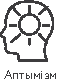
\includegraphics[scale=1.5]{willpower/ch7/15.pdf}
\end{figure}

\textbf{Трэнаваньне аптымізму} заключаецца ў~тым, каб сьвядома факусаваць увагу на станоўчых аспэктах, разглядаць іх у~аптымістычнай атрыбуцыі і памяняць стыль разгляду няўдачаў. Гэта можна рабіць, напрыклад, у~пісьмовым выглядзе. Іншыя спосабы ўключаюць кагнітыўныя трэніроўкі, напрыклад існуе праграма, у~якой вы на хуткасьць вызначаеце радасныя твары сярод сумных і нэўтральных. Пры вядзеньні дзёньніка важна сьвядома мяняць свой стыль апісаньня і факусавацца на станоўчых аспэктах таго, што адбываецца. Паспрабуйце пару дзён «пазітыўнай дыеты», калі вы глядзіце, чытаеце, думаеце толькі пазітыўныя рэчы і падзеі.

\textbf{Гумар і сьмех}~--- гэта выдатныя спосабы рэляксацыі і зьніжэньня стрэсу, а~здольнасьць пасьмяяцца зь сябе~--- важная ўмова здароўя і практык здароўя, таму часьцей жартуйце, сьмейцеся, глядзіце больш камедый і чытайце вясёлыя кнігі. 

\begin{figure}[htb!]
  \centering
  
\includegraphics[scale=1.5]{willpower/ch7/16.pdf}
\end{figure}

\emph{У дасьледаваньні прагляд камедый і фільмаў жахаў прывёў да розьніцы ў~50\,\% у~ступені пашырэньня сасудаў: гумар паляпшае аслабленьне сьценак артэрыяў. Таксама сьмех спрыяе выдзяленьню бэта-эндарфінаў, зьніжае боль, маркеры запаленьня. Яшчэ ў~60-х гадах XX стагодзьдзя былі закладзеныя асновы гелотатэрапіі~--- тэрапіі сьмехам, а~цяпер карыстаецца папулярнасьцю такі кірунак, як ёга сьмеху.}

Калі эўрапейцы ўпершыню ўзяліся за навуковае вывучэньне ўсходніх практык, то яны былі зьбітыя з~панталыку тым, што тыбэцкія будысты ўвесь час жартавалі зь іх. Эўрапейцы спрабавалі настойваць на сур'ёзнасьці, але ім патлумачылі, што пачуцьцё гумару~--- гэта абавязковая ўмова разуменьня складаных мэдытатыўных практык. І сёньня можна ўбачыць, як людзі «вельмі сур'ёзна» мэдытуюць або займаюцца здаровым харчаваньнем, што прыкметна павышае рызыку артарэксіі. 

Як зьвязаныя гумар і ўсьвядомленасьць? Абодва яны патрабуюць разгляду сытуацыі збоку, погляд мэта-назіральніка. А гэта магчыма пры актыўнай прэфрантальнай кары і пасавай зьвіліне, што ўжо гаворыць пра здароўе і зьніжэньне стрэсу. Калі вам ня сьмешна ані каліўца, то вы не ўсьвядомленыя ў~гэтай сытуацыі ні на грам. 

\emph{Мы часта сьмяёмся без нагоды, і гэта абсалютна нармальна, бо толькі 10\,\% сьмеху выклікана жартамі.}

Цікава, што гумар пры старэньні і нэўрадэгенэратыўных захворваньнях часта мяняецца самым першым, як складаная мазгавая функцыя. Таму зьмена пачуцьця гумару можа быць трывожным сымптомам.

\textbf{Сьмех расслабляе.} Яшчэ філёзаф Імануіл Кант прыкмеціў: «Сьмех ёсьць афэкт ад раптоўнага пераўтварэньня напружанага чаканьня ў~нішто». Сьмех робіць страшнае нястрашным. Таму многія людзі панічна баяцца сьмеху, баючыся, што сьмех пазбавіць іх «аўтарытэту». Для жанчынаў пачуцьцё гумару зьяўляецца важным крытэрам выбару партнёра. Сьмех у~пары дазваляе партнёрам хутчэй здымаць напружаньне пасьля цяжкіх падзей, і ў~цэлым сумеснае жыцьцё такой пары звычайна працягваецца даўжэй. Сьмех збліжае~--- гэта выдатная разрадка сытуацыі і сацыяльная эмоцыя, якая гуртуе людзей незалежна ад таго, ці быў жарт сьмешны. 

\textbf{Сьмех~--- гэта рэальны індыкатар блізкасьці.}

\textbf{Сьмех карысны для здароўя.} Ён зьніжае ўзровень картызолу, паляпшае імунную функцыю, падаўжае жыцьцё як здаровым, так і хворым. Згодна з~дасьледаваньнямі, сьмяротнасьць сярод хворых, якія маюць добрае пачуцьцё гумару, ніжэйшая на 31\,\%. 

\emph{У дасьледаваньнях паказана, што сьмех паляпшае адчувальнасьць да інсуліну: дыябэтыкі і здаровыя людзі елі, а~затым сядзелі на нуднай лекцыі ці на камэдыйным шоў. Пасьля шоў нават у~дыябэтыкаў уздым цукру быў мінімальны ў~параўнаньні з~тымі, хто слухаў лекцыю. У іншай працы паказана спрыяльны ўплыў сьмеху на рэнін-ангіятэнзінавую сыстэму: сьмех зьніжаў рэнін плазмы.}

\infobox{З узростам мы сьмяёмся ўсё менш: дзіця сьмяецца ў~20 разоў больш за дарослага. Страта гумару гаворыць пра непамысныя зьмены асобы. Зьмена пачуцьця гумару~--- прыкмета шматлікіх парушэньняў, напрыклад старэньня.}

\textbf{Сьмех дапамагае вучыцца.} Навукоўцы ўстанавілі, што дзеці, якіх сьмяшылі, лепш навучаюцца, а~дзеці, якія не рэагуюць на жарты, навучаюцца горш. Студэнты больш эфэктыўна запаміналі матэрыялы, калі выкладчыкі расказвалі нешта сьмешнае, зьвязанае з~тэмай урока. Калі я выкладаў у~мэдунівэрсытэце, то таксама актыўна выкарыстоўваў гэты прыём.

\subsection*{Кагнітыўная гнуткасьць}

Калі мы ўспрымаем сябе ў~сытуацыі стрэсу як цьвёрды камень, на якім расьце ноша, то адчуваем, што можам трэснуць і рассыпацца, калі нагрузка стане крытычнай. Так і бура можа з~коранем вырваць магутны дуб, а~вось гнуткая вярба прыгнецца да зямлі і выжыве. Калі перапаліць сталь, яна стане вельмі крохкай!

\begin{figure}[htb!]
  \centering
  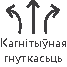
\includegraphics[scale=1.5]{willpower/ch7/17.pdf}
\end{figure}

\textbf{Гнуткасьць забясьпечвае нам запас трываласьці і лепшы кантроль над сваімі рэакцыямі.} Пры стрэсе нам вельмі часта шкодзіць зацыкленасьць. Мы можам шматкроць пракручваць траўмавальную сытуацыю або фіксавацца толькі на адным яе аспэкце, выпускаючы з-пад увагі ўсё астатняе. Павелічэньне кагнітыўнай гнуткасьці, г.~зн. здольнасьці пераключацца між сытуацыямі,~--- важны і карысны навык. 

\emph{Мазгавой структурай, якая забясьпечвае гнуткасьць, зьяўляецца зьвіліна поясу, перадусім пярэдняя яе частка. Гэта наша своеасаблівая каробка перадач мозгу, яна асабліва актыўная тады, калі для рашэньня задачы патрабуецца прыкласьці разумовае намаганьне або сканцэнтравацца, калі трэба пераключаць увагу з~аднаго аб'екта на іншы, з~адной думкі на іншую, бачыць розныя варыянты, правільна спраўляцца зь пераменамі.}

Кагнітыўная гнуткасьць забясьпечвае адначасовае абдумваньне мноства бакоў зьявы, бачаньне вялікай колькасьці розных аспэктаў сытуацыі, дапамагае зьмене ўстаноўкі і разуменьню разнастайных варыянтаў дзеяньня. Калі ў~чалавека нізкая кагнітыўная гнуткасьць, то ён зацыклены на сваіх праблемах, у~яго схільнасьць да абсэсіўна-кампульсіўных паводзінаў і працяглага ўтрыманьня траўмы ўнутры сябе, яму складана мяняцца і дамаўляцца з~людзьмі.

\textbf{Пастаянныя дрэнныя думкі пагаршаюць настрой, дрэнны настрой вядзе да пазьбяганьня патрэбных дзеяньняў, падае вера ў~сябе, дрэнных думак становіцца яшчэ больш~--- і гэтак далей па коле.} Або дрэнныя думкі прыводзяць да дрэннай ацэнкі іншых людзей, гэта пагаршае ўзаемадзеяньне, людзі рэагуюць нэгатыўна, што прыводзіць да яшчэ горшага іх ацэньваньня~--- і зноў па коле. Такіх сытуацый можа быць шмат, калі ня ўмець пераключацца.

\textbf{Для павышэньня кагнітыўнай гнуткасьці} важна ўмець адцягвацца, практыкаваць выпісваньне думак, прывучаць мозг да пастаяннага пошуку розных варыянтаў і опцый, новых ідэй~--- чым больш, тым лепш. Напрыклад, як з~пункта А трапіць у~пункт Б максімальна вялікай колькасьцю спосабаў? Дапамагаюць павысіць гнуткасьць камунікацыя і выслухоўваньне розных пунктаў гледжаньня. Карысна пасьмяяцца з~сябе, давесьці сытуацыю да абсурду, каб яна вас адпусьціла. Паспрабуйце рэфрэймінг сытуацыі: як бы да яе паставіліся іншыя людзі, як бы вы зрабілі праз 5, 20, 40 гадоў і да т.~п. Пэрыядычна выкідайце лішняе і наводзіце парадак~--- гэта таксама карысна для гнуткасьці. 

\infobox{Практыкуйце спантаннасьць~--- станцуйце, схадзіце ў~новае месца, зрабіце што-небудзь незвычайнае. Альтруізм, суперажываньне, дзеяньні ў~інтарэсах іншых, клопат пра іншых дапамагае стаць больш гнуткім, бо зацыкленасьць на сваіх асабістых перажываньнях робіць нас менш гнуткімі.}

\subsection*{Шанцунак}

Кожны дзень па ўсім сьвеце людзі пачынаюць мноства праектаў, але толькі малая частка зь іх становіцца пасьпяховымі. Гэта здаецца дзіўным, бо вакол нас мноства пасьпяховых бізнэсаў, якія, як бачыцца збоку, можна лёгка ўзяць і скапіяваць, шмат гатовых сакрэтаў посьпеху, шмат схэмаў, плянаў і стратэгій~--- бяры і рабі. Чаму ж гэта не працуе? Адказ заключаецца ў~асаблівасьцях працы мозгу прыдакаў і няўдакаў. \textbf{Тое, як працуе вашая зьвіліна поясу, уплывае на пасьпяховасьць і шанцунак, незалежна ад узроўню адукацыі, матывацыі або стартавага капіталу.}

\emph{Прафэсар Рычард Вайсман на працягу шматлікіх гадоў вывучаў, як працуе мозг людзей, якія лічаць сябе прыдакамі і няўдакамі. Напрыклад, ён раздаваў паддосьледным газэту і прасіў іх падлічыць колькасьць фатаграфій у~ёй. На другой старонцы газэты было вялікімі літарамі надрукавана, што ў~газэце 43 фатаграфіі, можна далей не чытаць. У іншых досьледах устаўлялі надпіс: ``Калі вы гэта чытаеце, то скажыце экспэрымэнтатарам, і атрымаеце 250 фунтаў''. Прыдачыкі заўважалі гэтыя надпісы, спыняліся і атрымлівалі сумы грошай, а~вось няўдакі працягвалі лічыць усе фатаграфіі да самага канца газэты і прапускалі фінансавую прапанову.}

\textbf{Фактар посьпеху} зьвязаны з~тым, што ўдачлівыя людзі маюць нашмат шырэйшы фокус увагі і не зацыкліваюцца на бягучым заданьні. Гэта дазваляе ім быць гнуткімі, хутка перабудоўвацца і аптымальным чынам выкарыстаць наяўныя рэсурсы. Удачлівыя людзі часьцей імкнуцца да нявызначанасьці і з~задавальненьнем спрабуюць новае і нязвыклае, пашыраюць сваё камунікатыўнае кола. Цікава, але прыдакі і пасьпяховыя людзі часьцей, чым няўдакі, памыляюцца, але вельмі хутка аднаўляюцца пасьля памылак. У няўдакаў фокус увагі вельмі вузкі, яны ігнаруюць і не заўважаюць нічога, акрамя іх бягучага заданьня. Такая фіксацыя робіць іх трывожнымі, зацыкленымі, мэтай іх дзеяньняў становіцца пазьбяганьне памылак. Яны пагарджаюць альтэрнатыўнымі магчымасьцямі і ня могуць зьмяніць свае паводзіны, адмаўляюцца ад усяго нязвыклага, звужаюць круг знаёмстваў, выбіраючы ``стабільнасьць'', ``быць як усё'' і ``што ж скажуць людзі?''. 

\infobox{Няўдакі шукаюць ``ідэальнае'' рашэньне, нейкі ``цуд'', сакрэт ад гуру, што будзе здольны вырашыць адразу ўсе іх праблемы за адзін падыход.}

Калі чарговы рэцэпт не спрацоўвае, няўдака ня робіць высноў, а~проста пераключаецца на іншы ``рэцэпт посьпеху''. Падобная кагнітыўная памылка называецца «памылкай выжылага» і тлумачыць, чаму не працуюць чужыя сакрэты посьпеху. 

\subsection*{Як зрабіць свой розум гнуткім?}

Важна дэталёва разгледзець усе ідэі, спосабы, у~тым ліку тыя, якія вам не падабаюцца. Калі вы адчуваеце, што зацыкліваецеся на нечым, важна своечасова пераключыцца, адпачыць. Практыкуйце шматварыятыўнасьць і стымулюйце крэатыўнасьць: заўсёды майце альтэрнатыўныя спосабы дасягненьня мэты. 

\emph{Празьмерныя стараньні пагаршаюць вашую эфэктыўнасьць. Закон оптымуму матывацыі Еркса-Додсана вястуе, што найлепшыя вынікі дасягаюцца пры сярэднім узроўні матывацыі. Пры гэтым чым складанейшая вашая задача, тым ніжэйшы ўзровень матывацыі патрэбны для прадуктыўнасьці. Г.зн. высокая матывацыя і напруга дапамогуць вам хутчэй выкапаць канаву, але ані не дапамогуць палепшыць працу кампаніі. Гумар, абсурдызацыя, парадокс, гульня і спантаннасьць дапамогуць вам стаць лягчэйшымі і спросьцяць жыцьцё.}

Як і любая іншая зьмена, паляпшэньне кагнітыўнае гнуткасьці пачынаецца з~усьведамленьня праблемы. Як толькі мы перастанем ваяваць з~рэальнасьцю, яна разгорне перад намі велізарную прастору магчымасьцяў. Трэба расплюшчыць вочы, каб убачыць дары рэальнасьці. І чым гнутчэйшы наш мозг, тым лягчэй нам да іх дацягнуцца.

\textbf{Займайцеся творчасьцю!} Дасьледаваньні паказваюць, што многія праявы спантаннасьці, такія як экспрэсіўнае пісьмо, музыка, танец і арт-тэрапія паляпшаюць агульны стан чалавека, павышаюць стрэсаўстойлівасьць, зьніжаюць узровень картызолу. Арт-тэ\-ра\-пію хоць і разглядаюць як ``сублімацыю'', мне здаецца, лепш успрымаць гэтую мэтодыку як разнавід пошукавай актыўнасьці.

\emph{Арт-тэрапія~--- выдатны неканкурэнтны від дзейнасьці, які павышае актыўнасьць зьвіліны поясу, які зьніжае румінацыю. Ён паляпшае канцэнтрацыю ўвагі, дапамагае вырашыць унутрыасобасныя канфлікты і зьмяніць звыклыя паводзінныя стэрэатыпы.}

\begin{figure}[htb!]
  \centering
  
\includegraphics[scale=1.5]{willpower/ch7/18.pdf}
\end{figure}

\textbf{Пры стрэсе выбар невялікі: альбо вывучаная бездапаможнасьць, альбо пошукавая актыўнасьць.} Усё, што стымулюе новыя віды дзейнасьці, карыснае. Галоўнае~--- ня блытаць спантаннасьць і творчасьць з~імпульсіўнасьцю і няўстойлівасьцю ўвагі, гэта зусім розныя працэсы. Часта можна ўбачыць, што дэфіцыт увагі і гіпэрактыўнасьць успрымаюцца як ``творчыя імпульсы'', але гэта ня так.

Сачыненьне, маляваньне, ігра на інструмэнтах~--- усё працуе выдатна, нават калі ў~вас ``пасрэдны'' ўзровень. Таму, калі адчуваеце стрэс, займіцеся творчасьцю ці выявіце спантаннасьць любым са спосабаў. Дастаткова 45 хвілінаў творчасьці, каб прыкметна зьнізіць узровень картызолу. 

\emph{Нам зь дзецьмі цяпер лепш за ўсё пасуе драма~--- экспрэсіўнае разыгрываньне роляў і сюжэтаў, ад коцікаў да трансформэраў.}

\subsection*{Пытаньні і заданьні}

1. Патрэніруйцеся аптымістычна рэагаваць на сытуацыі, як удалыя, так і няўдалыя. Спытайце сябе, што б падумаў аптыміст, ацэньваючы пастаянства, унівэрсальнасьць, пэрсаналізацыю праблемы.

2. Калі вы пачынаеце зацыклівацца на праблеме~--- адцягвайцеся. Што эфэктыўна пераключыць вашу ўвагу? Планка? Тэтрыс?

3. Заплянуйце дзень сьмехатэрапіі. Якія жарты, камэдыі, комікі і шоў сьмяшаць вас мацней за ўсё?


\section{Цялесныя рэсурсы стрэсаўстойлівасьці. Вагус і аксытацын}

Калі я вяду курс «Стрэсаўстойлівасьць», я цытую Айнштэйна, які казаў, што «немагчыма вырашыць праблему на тым жа ўзроўні, на якім яна ўзьнікла». Для таго каб даць рады стрэсу, можна падысьці «зьверху», праз псыхічныя рэсурсы стрэсаўстойлівасьці, якія мы разабралі. Але можна падысьці і «зьнізу», узьдзейнічаючы на цела. Аптымальна, вядома, спалучаць гэтыя падыходы.

Часьцяком, калі мы ня можам вырашыць праблему проста, то выкарыстоўваем \textbf{зрушаную актыўнасьць}, успомніце, напрыклад, сцэну з~начной колкаю дроваў у~фільме «Утаймаваньне свавольніка».

Зрушаная актыўнасьць узьнікае, калі ёсьць магутная матывацыя штосьці зрабіць, але ўмовы не дазваляюць, ці калі ёсьць некалькі супярэчлівых матывацый, і абраць дзеяньне цяжка. Часта зрушаная актыўнасьць узьнікае ў~новай сытуацыі, калі няма гатовага рашэньня, і часьцей за ўсё такое дзеяньне будзе біялягічна не мэтазгоднае. Жывёлы пры стрэсе могуць імітаваць засынаньне, другія пачынаюць мыцца, трэція пазяхаць~--- г.~зн. дзейнічаць «зрушана», не па сытуацыі.

Людзі таксама праяўляюць сябе па-рознаму: мы чухаем галаву, трымаемся за падбародзьдзе, круцім пярсьцёнак, мыем і без таго чыстыя паверхні, выцягваем вусны, грызём аловак. Часам паступаем зусім дзіўна: зрываемся на іншых людзях, увязваемся ў~чужыя справы і да т.~п. Такая рэакцыя не вырашае праблему, але дапамагае нам «зрабіць паўзу», палегчыць сымптомы стрэсу, а~пры стрэсе любая актыўнасьць лепш, чым проста ляжаць на канапе. 

\infobox{Калі стрэс высокі, а~зрабіць нічога нельга, зьвярніце сваю ўвагу на цела.}

Як мы ўжо з~вамі ведаем, сымпатыйная нэрвовая сыстэма адказвае за стрэсавую рэакцыю, а~парасымпатыйная за зьніжэньне стрэсу, гэта пэдаль тормазу стрэсавай рэакцыі. 

Актывацыя парасымпатыйнае сыстэмы вядзе да зьніжэньня пульсу, ціску, пачырваненьня скуры, да паляпшэньня страваваньня і да т.~п. І тут добра працуюць вагус (блукальны нэрв) і гармон аксытацын. Аксытацын стымулюе тонус вагуса, таму для зручнасьці мы будзем разглядаць «вагусныя» і «аксытацынавыя» спосабы стымуляцыі разам.

\subsection*{Роля аксытацыну}

\textbf{Аксытацын}, апроч іншых сваіх уласьцівасьцяў, яшчэ і антыстрэсавы гармон. Ён выклікае пачуцьцё задавальненьня, зьніжэньне трывогі і пачуцьцё спакою, павялічвае давер і зьніжае страх. Яшчэ аксытацын зьніжае апэтыт і амалоджвае цягліцы. 

\emph{Дзеяньне аксытацыну мае гендэрную розьніцу. Калі мужчына кажа «адчапіся ад мяне~--- у~мяне стрэс», то жанчына~--- «пагавары са мной~--- у~мяне стрэс». Мужчынам павышэньне тэстастэрону дапамагае лягчэй пераадолець стрэс, а~аксытацын можа яшчэ ніжэй апусьціць узровень тэстастэрону. А вось у~жанчынаў аксытацын пры стрэсе працуе ідэальна.}

\begin{figure}[htb!]
  \centering
  
\includegraphics[scale=1.5]{willpower/ch7/19.pdf}
\end{figure}

Аксытацын стымулюецца пры любых спосабах сацыяльнага ``аб'яднаньня'', калі мы адчуваем сувязь з~кім-небудзь. Нават бескантактавыя спосабы, такія як пачуцьцё прыналежнасьці да нечага, позірк у~вочы і камплімэнты, павялічваюць выдзяленьне аксытацыну. Асабліва магутна выклікаюць выкід аксытацыну маленькія дзеці~--- узьнікае замілаваньне і расслабленьне. 

Большасьць цялесных спосабаў рэляксацыі так ці інакш уплываюць на актыўнасьць парасымпатыйнай нэрвовай сыстэмы. Галоўным нэрвам парасымпатыйнай сыстэмы зьяўляецца вагус, які злучае ўнутраныя органы і мозг, нясе інфармацыю пра стан цела. 

\subsection*{Роля вагус}

Актыўнасьць вагуса вызначаецца яго тонусам, які паказвае, наколькі хутка наша цела можа пераходзіць са стану стрэсу ў~расслаблены стан. Чым ніжэйшы тонус вагуса, тым складаней нам расслабляцца і тым мацней стрэс дзейнічае на наша цела, павялічваючы рызыкі сардэчна-сасудзістых захворваньняў, дыябэту і атлусьценьня, узроўню запаленьня і інш. Нармальны тонус вагуса зьвязаны зь лепшым псыхічным і фізычным здароўем, рэсурсам адаптацыі да вонкавых абставінаў..

Проста зараз зрабіце просты досьлед. Набярыце ракавіну халоднай вады (можна кінуць крыху лёду), памерайце свой пульс. Затым глыбока ўдыхніце і пагрузіце твар. Памерайце пульс зноў~--- ён прыкметна запаволіўся, а~вы супакоіліся. Гэта старажытны ныральны рэфлекс, які працуе праз блукальны нэрв, які актывуе парасымпатыйную антыстрэсавую сыстэму.

\textbf{Існуе некалькі гіпотэзаў аб уплыве вагуса на здароўе.} Тэорыя Тэера кажа, што вагус уплывае на стрэсаўстойлівасьць і эмацыйны стан і можа вызначаць працягласьць жыцьця і сярэдні IQ. Тэорыя Трэйсі вястуе, што вагус прыгнятае сыстэмнае хранічнае запаленьне і тым самым карысны. Мэдыятарам парасымпатыйнай сыстэмы зьяўляецца ацэтылхалін, які можа зьніжаць узровень запаленьня і рызыку многіх захворваньняў, ад дэпрэсіі да аўтаімунных.

\emph{Алькалёіды, якія ўтрымліваюцца ў~пасьлёнавых (перац, таматы, баклажаны і інш.), стымулююць тонус вагуса і зьніжаюць узровень запаленьня ў~арганізьме. Алькалёіды з~пасьлёнавых падобныя па ўзьдзеяньні на нікатынам. Навукоўцы ўсталявалі, што нікатын зьніжае рызыку хваробы Паркінсана, памяншае праявы дэфіцыту ўвагі і гіпэрактыўнасьці, а~таксама частасьць і выяўленасьць сымптомаў шэрагу аўтаімунных хваробаў. Узьдзеяньне нікатыну на дафамінавыя рэцэптары, якія гінуць пры хваробе Паркінсана, даведзенае як для людзей, так і для жывёл. Кожная порцыя пасьлёнавых на 31\,\% можа зьніжаць рызыку хваробы Паркінсана. Наймацнейшы ахоўны эфэкт назіраецца ў~салодкага перцу: хто есьць перцы пяць разоў на тыдзень, захворвае на 50\,\% радзей, чым тыя, хто ўжывае іх менш разу на тыдзень.}

Тонус вагуса ўплывае і на нашыя \textbf{сацыяльныя паводзіны}: чым больш у~нас сацыяльных кантактаў, чым больш пазітыву ў~камунікацыі, тым вышэйшы тонус вагуса. А чым вышэйшы тонус, тым больш мы маем камунікуем, -- узьнікае чарговае замкнёнае кола. Нізкі тонус вагуса зьвязаны з~кепскім настроем і пачуцьцём адзіноты. Вызначыць тонус вагуса можна, напрыклад, ацэньваючы ўзровень дыхальнай арытміі~--- гэта невялікае павышэньне пульсу пры ўдыху і зьніжэньне на выдыху. Зручнейшым зьяўляецца вымярэньне тонусу вагуса праз варыябельнасьць пульсу, што даступна ў~шматлікіх праграмах. Чым больш у~нас сацыяльных кантактаў, тым вышэйшы тонус вагуса. Нізкі тонус вагуса зьвязаны з~кепскім настроем і адчуваньнем самоты.

\begin{figure}[htb!]
  \centering
  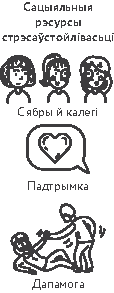
\includegraphics[scale=1.5]{willpower/ch7/20.pdf}
\end{figure}

\textbf{Сацыяльныя рэсурсы.} У адным з~дасьледаваньняў навукоўцы раілі кожны дзень запісваць тры сацыяльныя кантакты і ацэньваць іх, згаджаючыся ці абвяргаючы сьцьверджаньні: ``я адчуваў гармонію з~гэтым чалавекам пры камунікацыі'' і ``я адчуваў блізкасьць з~гэтым чалавекам пры камунікацыі''. А таксама ім раілі ацэньваць па пяцібальнай шкале ўзровень станоўчых (удзячнасьць, надзея, натхненьне, радасьць, цікавасьць, любоў, гонар, спакой, зьдзіўленьне, пашанота) і адмоўных эмоцыяў (злосьць, нуда, агіда, пагарда, зьбянтэжанасьць, страх, віна, нянавісьць, смутак, сорам) з~падлікам сярэдніх значэньняў. Высьветлілася, што эмацыйная ўсьвядомленасьць, то бок здольнасьць разьбірацца ў~сваіх эмоцыях, прыкметна павялічвае тонус вагуса. Падрабязна пра ўсьвядомленасьць пагаворым у~наступным разьдзеле. У дасьледаваньнях устаноўлена, што рэгулярная мэдытацыя дабрыні й любові павышае тонус вагуса. Таму гадуйце ў~сабе пачуцьці любові, добразычлівасьці, спагады да навакольных~--- гэта карысна і вам.

Камплімэнты, абдымкі, знаходжаньне ў бясьпечным асяродзьдзі, погляд вочы ў~вочы, пацалункі, абдымкі, сэкс. Паціскаць можна і цацкі, і хатніх жывёл, а~можна і паплакаць~--- гэта таксама актывуе вагус. Пацалунак ня меншы за 6 сэкундаў, абдымкі ня меншыя за 20 сэкундаў будуць найболей карысныя.

\subsection*{Рэгулярная фізычная актыўнасьць}

Рухальная актыўнасьць імітуе натуральны эвалюцыйны мэханізм «бі--бяжы» і дапамагае прыбраць лішнія глюкозу і тлушчы, якія цыркулююць у~крыві. Для спартоўцаў і аматараў характэрны высокі тонус вагуса. Цяглічная актыўнасьць павышае ўзровень нэўратрафічнага чыньніка BDNF, што павышае нэўраплястычнасьць і нашыя шанцы супрацьстаяць стрэсу, разьвіваць новыя навыкі. На гэта лепш за ўсё працуюць аэробныя практыкаваньні з~60--70\,\% узмацненьнем рытму сэрца ня менш за 30 хвілінаў. Зрэшты, пасуе і кароткая інтэнсіўная нагрузка: тры хвіліны спрынту на 20\,\% павялічваюць кагнітыўныя здольнасьці. Наагул скачкі, спантанная актыўнасьць і танцы паднімаюць BDNF нашмат мацней у~параўнаньні з~фітнэсам.

\subsection*{Цяглічны тонус}

Пры стрэсе назіраецца ўзмацненьне цяглічнага тонусу, а~такі стан заціснутасьці некамфортны. Цяглічныя рэляксацыі і расьцяжкі могуць дапамагчы з~гэтым. 

\emph{Напрыклад, прагрэсіўная цяглічная рэляксацыя, дзе выкарыстоўваецца напруга цягліц, якая затым прыводзіць да іх паслабленьня. Пасьлядоўнасьць такая: напружваем ручыцы і перадплеччы (трэба моцна сьціснуць кулакі, паклаўшы вялікія пальцы зьверху), верхнія цягліцы рук (уціснуць локці ў~сьпінку крэсла або стол), твар (падняць бровы, заплюшчыць вочы, наморшчыць нос, зрабіць усьмешку з~апушчанымі куточкамі вуснаў), шыю (уціснуць падбародак у~вобласьць адамава яблыка), тулава (адвесьці лапаткі назад і моцна прагнуць сьпіну), ногі (падняць уверх і напружыць, пальцы ў~падлогу, затым тое ж самае, але пальцы ў~столь). У кожным сьціску затрымайцеся на некалькі удыхаў, а~затым зрабіце павольны выдых, расслабляючы цягліцы.}

Таксама фізычная актыўнасьць павялічвае тонус вагуса, зьмяншае пульс супакою. Чым больш вы трэніраваныя, тым больш стрэсаўстойлівыя. А акрамя гэтага, фізычная актыўнасьць~--- гэта найлепшы спосаб завяршэньня стрэсавай рэакцыі і яе наступстваў. Бо для нашага цела любы стрэс~--- гэта фізычная актыўнасьць, ``бі або бяжы''.

\begin{figure}[htb!]
  \centering
  
\includegraphics[scale=1.5]{willpower/ch7/21.pdf}
\end{figure}

\subsection*{Аўтагенная трэніроўка}

Гэта просты і эфэктыўны спосаб рэляксацыі, заснаваны на візуалізацыі. Пачынаючы з~ручыцаў і ступакоў, далей рухаючыся па ўсім целе, мы па чарзе ўяўляем у~іх «цяжар»~--- на расслабленьне цяглічнага тонусу, і «цяпло»~--- на пашырэньне сасудаў скурнага покрыва. Візуалізацыя прахалоды на лобе можа дапамагчы ў~аслабленьні галаўнога болю.

\subsection*{Дыхальныя практыкі}

Пры стрэсе ў~нас запускаецца мэханізм пачашчэньня дыханьня. Гэта адаптыўны мэханізм, гатоўнасьць арганізма да «бегчы-біцца». У чым фізыялягічны мэханізм гэтай зьявы? Гіпэрвэнтыляцыя~--- гэта прыстасоўвальны эвалюцыйны стрэсавы мэханізм. Пры зьніжэньні CO\textsubscript{2} павялічваецца ўзровень ўнутрыклеткавага кальцыю. Гэта актывуе скарачальныя ўласьцівасьці ўсіх цяглічных тканак, узмацняе цяглічную напругу, павялічвае адчувальнасьць рэцэптараў да адрэналіну. Таму павольнае дыханьне рэальна расслабляе, зьніжаючы цяглічны тонус і адчувальнасьць да адрэналіну.

\begin{figure}[htb!]
  \centering
  
\includegraphics[scale=1.5]{willpower/ch7/22.pdf}
\end{figure}

\emph{Гіпэрвэнтыляцыя вядзе да павелічэньня скарачальнай актыўнасьці і шкілетных цягліцаў, і гладкіх цягліцаў сасудаў. Але самае важнае~--- гэта вымываньне вуглякіслага газу з~крыві, што прыводзіць да звужэньня крывяносных сасудаў у~галаўным мозгу і выклікае зьніжэньне крывацёку. Гэта можа прыводзіць да галавакружэньня, звужэньня прытомнасьці, зьніжэньня ўвагі, паколваньня, здранцьвеньня, спазмаў, часам выяўляецца як адчуваньне здушваньня ў~грудзях, як ком у~горле і да т.~п.}

Спакойнае мернае глыбокае дыханьне зьніжае актыўнасьць сымпатыйнай стрэсавай сыстэмы і павышае актыўнасьць парасымпатыйнай, стымулюе блукальны нэрв і запавольвае частасьць сардэчных скарачэньняў.

\textbf{Для расслабляльнага дыханьня патрэбныя:} кароткі ўдых, доўгі выдых (у некалькі разоў даўжэйшы за ўдых), глыбокае павольнае дыяфрагмальнае дыханьне, затрымкі на выдыху ў~межах камфорту. Можна лічыць пра сябе, напрыклад удых на 4 лікі, выдых на 8 лікаў, затрымка на выдыху на 6 лікаў. Такое ``ўсьвядомленае дыханьне'' на лік дапамагае пры шматлікіх захворваньнях, паляпшае сон, зьніжае ціск, паляпшае ўвагу. 

Пры неабходнасьці скарыстайцеся праграмамі для дыханьня~--- іх цяпер мноства, і трымайце абразок праграмы на галоўным экране смартфона, так вам будзе прасьцей згадаць пра неабходнасьць ``падыхаць''.

\subsection*{Электрастымуляцыя вагуса}

Апошнім часам атрымала распаўсюджваньне празскурная стымуляцыя вагуса простымі прыборамі, у~тым ліку і для хатняга выкарыстаньня. Яна прызначаная для барацьбы зь мігрэньню, дэпрэсіяй (уключаючы працяглую, цяжкую, устойлівую да антыдэпрэсантаў), эпілепсіяй, экспэрымэнтальна выкарыстоўваецца як частка супрацьзапаленчай і антыстрэсавай тэрапіі.

\textbf{Прапрацоўка мяккіх тканак.} Людзі здавён-даўна практыкавалі лазьні, водныя працэдуры, масаж як спосабы палепшыць сваё здароўе і самаадчуваньне. Практычна ўсе падыходы, накіраваныя на цягліцы і скуру, надкосьніцу, карысныя пры стрэсе, стымулююць тонус вагуса і выдзяленьне аксытацыну. Гэта стараннае расьціраньне цела ручніком або шчоткай для цела, прапрацоўка валікам мяккіх тканак, усе віды масажаў, акупунктура, расчэсваньне валасоў, касмэталягічныя працэдуры і СПА. 

\begin{figure}[htb!]
  \centering
  
\includegraphics[scale=1.5]{willpower/ch7/23.pdf}
\end{figure}

\emph{Малпы выкарыстоўваюць грумінг~--- расчэсваньне~--- як спосаб зьніжэньня стрэсу і паляпшэньня сацыяльных сувязяў.}

\emph{Пацалунак не меней за шэсць сэкундаў, абдымкі не меней за 20 сэкундаў будуць найболей карысныя.}

\textbf{Харчаваньне.} Частае дробавае харчаваньне, вялікая колькасьць бялку і цукру, лішак высокаглікемічных вугляводаў стымулююць mTOR і спрыяюць павелічэньню актыўнасьці сымпатыйнай сыстэмы. Таму цалкам можна сказаць, што ``ты такі нэрвовы празь мяса''. Дбайнае перажоўваньне, нізкая ўдзельная шчыльнасьць ежы (агародніна, зеляніна), ежа ў~сямейным або сяброўскім коле, рэгулярны фастынг, адсутнасьць перакусаў, вялікая доля тлустай ежы спрыяюць паляпшэньню тонусу вагуса. 

\emph{Ёсьць зьвесткі, што даданьне амэга-3, цынку, лакта- і біфідабактерій, пра- і прэбіётыкаў можа таксама дапамагаць.}

\textbf{Загрызіце свой стрэс!} На курсе, прысьвечаным харчаваньню, я шмат расказваю пра важнасьць жаваньня, на стрэсаўстойлівасьць гэты працэс таксама ўплывае. Жаваньне зьяўляецца дзейснай стрэсавай копінг-стратэгій, а~пры лішку стрэсу часта назіраецца бруксізм~--- скрыгат зубамі ў~сьне, які павялічвае рызыку карыесу ды іншых праблемаў. Дасьледаваньні паказваюць, што жаваньне зьніжае ўзровень выдзяленьня норадрэналіну ў~мігдаліне, узроўні АКТГ і картызолу, таксама зьніжае актыўнасьць стрэсавай восі, дзейнічаючы праз картызолавыя рэцэптары ў~гіпакампе, і кагнітыўны дэфіцыт, выкліканы стрэсавым пашкоджаньнем гіпакампа.

Чым больш інтэнсіўнае жаваньне, тым больш прыкметна зьніжаецца ўзровень картызолу і адрэналіну: хуткае жаваньне зьніжае ўзровень картызолу на 26\,\% за 20 хвілінаў. Што жаваць? Аптымальна гэта цьвёрдая ежа, напрыклад, морква ці яблык,~--- усе вынікі можна перанесьці й на жуйку.

\textbf{Завядзіце сабаку.} Наяўнасьць хатніх жывёлаў мае куды больш дадатных, чым адмоўных аспэктаў. Мы можам казаць нават пра PAT, або Реts As Therapy, дзе фэлінатэрапія~--- лячэньне коткамі, а~каністатэрапія~--- лячэньне сабакамі. Сацыяльнае ўзьдзеяньне зьвязанае з~тым, што хатнія жывёлы стымулююць камунікацыю, клопат, цялесныя кантакты, і гэта станоўча ўплывае на стрэсаўстойлівасьць. Так, рызыка інфаркту ва ўладальнікаў катоў на 30\,\% меншая, чым у~тых, хто жыве бяз хатніх жывёл. Сабакі таксама станоўча ўплываюць як на зьніжэньне рызыкі сардэчна-сасудзістых захворваньняў, так і на артэрыяльны ціск і нават на ліпідны профіль крыві.

\infobox{Дастаткова некалькіх хвілінаў камунікацыі паміж гаспадаром і сабакам для зьніжэньня ўзроўню картызолу~--- і ў~сабакі, дарэчы, таксама.}

\subsection*{Пытаньні і заданьні}

1. Схадзіце на масаж.

2. Паспрабуйце дыхальныя практыкі~--- яны вельмі эфэктыўныя і дзейнічаюць хутка. Усталюйце на тэлефон «дыхальную» праграму.

3. Пры стрэсе купіце моркву сярэдніх памераў і старанна яе згрызіце. Палягчэла?


\clearpage
\thispagestyle{empty}
\begin{figure*}[htb!]
  \vspace*{-0.5in}
  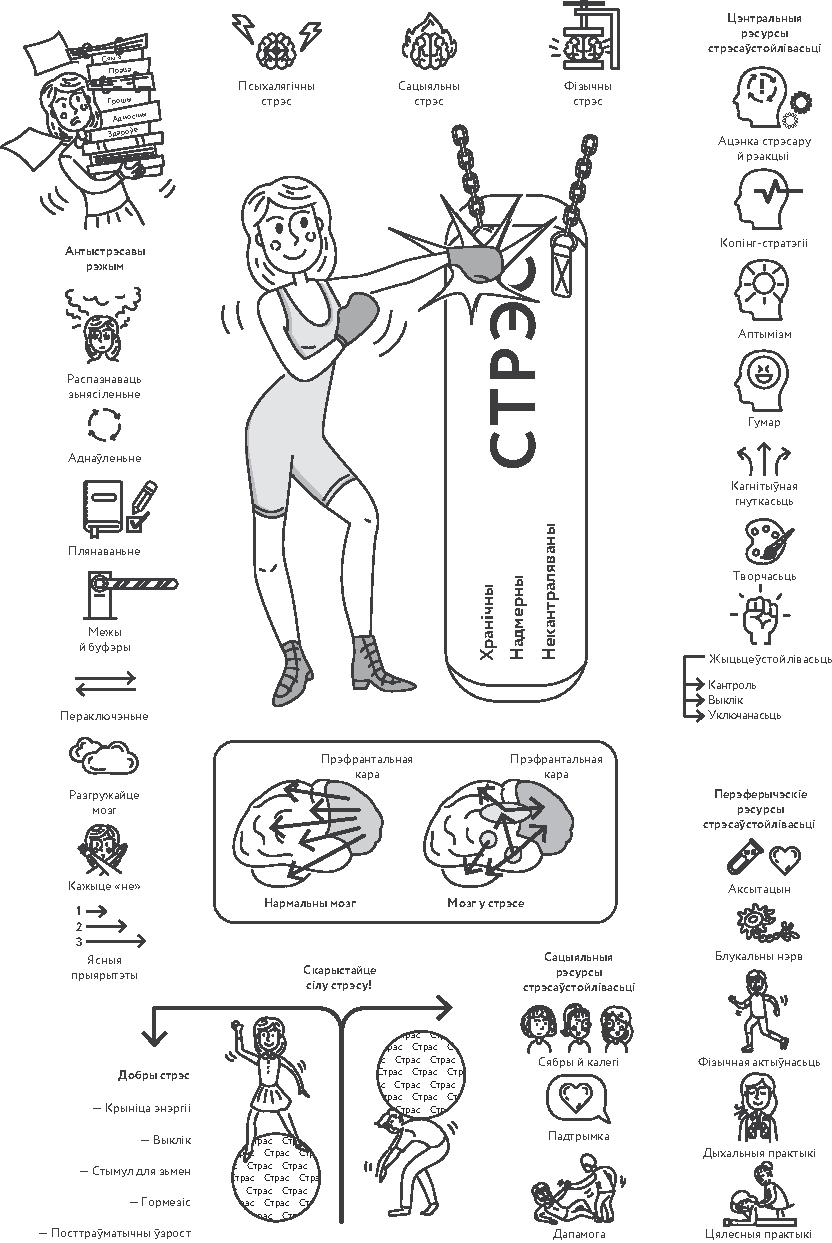
\includegraphics[width=0.95\textwidth]{willpower/ch7/full.pdf}  
\end{figure*}
